\documentclass[12pt,a4paper]{article}

% ─── Packages ────────────────────────────────────────────────────────────────
\usepackage[margin=1in]{geometry}
\usepackage{amsmath, amssymb}
\usepackage{graphicx}
\usepackage{booktabs}
\usepackage{array}
\usepackage{longtable}
\usepackage{multirow}
\usepackage{xcolor}
\usepackage{hyperref}
\usepackage{float}
\usepackage{caption}
\usepackage{subcaption}
\usepackage{setspace}
\usepackage{parskip}
\usepackage{enumitem}
\usepackage{fancyhdr}
\usepackage{titlesec}
\usepackage{authblk}
\usepackage{abstract}
\usepackage{microtype}
\usepackage{lmodern}
\usepackage[T1]{fontenc}
\usepackage[utf8]{inputenc}
\raggedbottom
% \colname{} — typewriter column name that allows line breaks at underscores/dots
\newcommand{\colname}[1]{{\ttfamily\renewcommand{\_}{\textunderscore\allowbreak}#1}}

% ─── Color Definitions ───────────────────────────────────────────────────────
\definecolor{navy}{RGB}{21,69,128}
\definecolor{lightblue}{RGB}{144,202,249}
\definecolor{darkred}{RGB}{183,28,28}
\definecolor{highlight}{RGB}{255,248,220}

% ─── Hyperref Setup ──────────────────────────────────────────────────────────
\hypersetup{
  colorlinks=true,
  linkcolor=navy,
  citecolor=navy,
  urlcolor=navy,
  pdftitle={Email Delivery A/B Experiment: Optimizing Funding Rate for Fintech Users},
  pdfauthor={Data Science Team}
}

% ─── Header / Footer ─────────────────────────────────────────────────────────
\pagestyle{fancy}
\fancyhf{}
\fancyhead[L]{\small\textcolor{navy}{Email A/B Experiment — Funding Rate Optimization}}
\fancyhead[R]{\small\textcolor{navy}{Executive Report}}
\fancyfoot[C]{\thepage}
\renewcommand{\headrulewidth}{0.4pt}
\renewcommand{\footrulewidth}{0.4pt}

% ─── Section Styling ─────────────────────────────────────────────────────────
\titleformat{\section}{\large\bfseries\color{navy}}{\thesection}{1em}{}
\titleformat{\subsection}{\normalsize\bfseries\color{navy}}{\thesubsection}{1em}{}
\titleformat{\subsubsection}{\normalsize\itshape\color{navy}}{\thesubsubsection}{1em}{}

% ─── Table Column Types ──────────────────────────────────────────────────────
\newcolumntype{L}[1]{>{\raggedright\arraybackslash}p{#1}}
\newcolumntype{C}[1]{>{\centering\arraybackslash}p{#1}}
\newcolumntype{R}[1]{>{\raggedleft\arraybackslash}p{#1}}

% ─── Spacing ─────────────────────────────────────────────────────────────────
\setstretch{1.3}
\setlength{\parskip}{6pt}
\emergencystretch=30pt  % allow extra stretch to avoid overfull hboxes in paragraphs

% ─── Graphics Path ───────────────────────────────────────────────────────────
\graphicspath{{../assets/}}

% ─────────────────────────────────────────────────────────────────────────────
%  DOCUMENT START
% ─────────────────────────────────────────────────────────────────────────────
\begin{document}

% ─── Title Page ──────────────────────────────────────────────────────────────
\begin{titlepage}
  \centering
  \vspace*{1.5cm}

  {\LARGE\bfseries\color{navy}
    Email Delivery A/B Experiment: \\[0.4em]
    Optimizing Funding Rate for Fintech Users
  }

  \vspace{1cm}
  \rule{\linewidth}{1.5pt}
  \vspace{0.5cm}

  {\large\textit{A Production-Grade Multi-Arm Experiment Analysis}}

  \vspace{1.5cm}

  \begin{tabular}{ll}
    \textbf{Team:}        & Data Science — Growth \& Engagement \\
    \textbf{Project:}     & Email Delivery Experiment on Funding Rate Improvement \\
    \textbf{Dataset:}     & 480,000 Users $\times$ 10 Templates $\times$ 24 Treatment Arms \\
    \textbf{Experiment:}  & 2020-11-30 (Day 0) through Day 32 (5-week duration) \\
    \textbf{Analysis:}    & February 2021 \\
    \textbf{Status:}      & Daily groups complete; Weekly groups pending final email \\
  \end{tabular}

  \vspace{2cm}

  \colorbox{highlight}{%
    \parbox{0.85\textwidth}{%
      \centering
      \textbf{Executive Summary:} 7 of 24 treatment arms show statistically significant
      improvement in funding rate ($p \leq 0.05$). Daily email delivery outperforms
      twice-a-week cadence. The \texttt{ml\_funding\_faq} template achieves the highest
      open rate ($\sim$31.5\%), 60\% above the campaign average.
      An estimated \textbf{500+ incremental funded users} are attributable to email intervention
      across significant groups.
    }
  }

  \vfill

\end{titlepage}

% ─── Table of Contents ───────────────────────────────────────────────────────
\tableofcontents
\clearpage

% ─────────────────────────────────────────────────────────────────────────────
\section{Introduction \& Business Context}
% ─────────────────────────────────────────────────────────────────────────────

\subsection{Business Problem}

In the competitive landscape of retail investing platforms — encompassing companies
such as Webull, Robinhood, Public, and Square's Cash App Investing — the
\textbf{account funding rate} represents one of the most operationally critical
conversion metrics. Formally, the funding rate is defined as:

\begin{equation}
  \text{Funding Rate} = \frac{|\text{Users who completed first deposit}|}{|\text{Users with approved accounts}|}
\end{equation}

\noindent where the numerator counts users whose \colname{first\_funded\_at} timestamp is
non-null (i.e., at least one deposit was completed), and the denominator counts all
approved accounts enrolled in the experiment.

A substantial proportion of users successfully complete the account approval process
but never take the final step of depositing funds and initiating investment activity.
This \textbf{funding gap} represents a direct revenue shortfall, as most retail investing
platforms monetize through trading commissions, payment for order flow (PFOF), or
margin lending — all of which require funded, active accounts.

Internal analysis identified three primary barriers preventing approved users from funding:

\begin{enumerate}[leftmargin=2em]
  \item \textbf{Knowledge barriers}: Users lack clarity on the funding mechanism,
    minimum deposit requirements, or the investment onboarding process.
  \item \textbf{Trust and safety concerns}: Users express hesitation about linking
    bank accounts or transferring funds to a relatively new platform.
  \item \textbf{Engagement decay}: Users who completed approval during a high-intent
    moment (e.g., a market event, promotional campaign) lose momentum before funding.
\end{enumerate}

\subsection{Proposed Solution: Personalized Email Intervention}

Marketing email remains one of the highest-ROI re-engagement channels for financial
services, offering direct, personalized communication with measurable behavioral tracking
(opens, clicks, conversions). The Growth team proposed a \textbf{multi-arm email experiment}
to systematically evaluate whether targeted email content could causally lift the
funding rate across different user behavioral segments.

The experiment's core hypothesis is:

\begin{quote}
  \textit{Email is the most effective channel to reach approved, unfunded users. The
  inventory of messages is exhaustive and directly addresses the concerns that hold
  users back from funding their accounts. We expect meaningful impact on email open
  rate, link rate, and funding rate across multiple user segments.}
\end{quote}

\subsection{Scope \& Objectives}

The experiment was scoped to address four primary business questions:

\begin{enumerate}[leftmargin=2em]
  \item \textbf{Content effectiveness}: Which of the 10 ML-generated email templates
    achieves the highest open rate? Does this vary by user segment?
  \item \textbf{Causal attribution}: Does receiving emails \textit{causally} increase
    funding rate, or do high-intent users self-select regardless?
  \item \textbf{Segment responsiveness}: Which user behavioral segments are most
    amenable to email-driven activation?
  \item \textbf{Delivery optimization}: Does daily vs.\ twice-a-week delivery frequency
    significantly impact outcomes?
\end{enumerate}

\clearpage
% ─────────────────────────────────────────────────────────────────────────────
\section{Data Description}
% ─────────────────────────────────────────────────────────────────────────────

\subsection{Dataset Overview}

The analysis pipeline ingests five structured datasets produced at different stages
of the experiment lifecycle — from experiment design through delivery tracking to
outcome measurement. Table~\ref{tab:datasets} provides a high-level summary; the
following subsections document each file's schema, column semantics, and role in
the analysis.

\begin{table}[H]
  \centering
  \caption{Dataset Summary}
  \label{tab:datasets}
  \resizebox{\textwidth}{!}{%
  \begin{tabular}{@{}L{5cm}C{2.5cm}L{7.5cm}@{}}
    \toprule
    \textbf{File} & \textbf{Shape} & \textbf{Role in Analysis} \\
    \midrule
    \colname{sample\_segment\_groups.csv}    & $12 \times 8$            & Defines the 12 behavioral user segments; maps segment IDs to feature flags and pool sizes \\
    \colname{sample\_uuid\_email\_order.csv} & $480{,}000 \times 13$    & Per-user randomized email delivery schedule; used for time-series pivot and delivery-order analysis \\
    \colname{email\_events.csv}              & $9{,}553{,}330 \times 6$ & Raw Post-Office event log; used for deliverability health checks and event volume breakdown \\
    \colname{user\_events.csv}               & $480{,}000 \times 22$    & Primary analysis table: per-user email status, account outcomes, and activity metrics \\
    \colname{control\_groups\_rate.csv}      & $12 \times 6$            & Pre-computed control group baseline funding and link rates; used as denominator in A/B z-tests \\
    \bottomrule
  \end{tabular}%
  }
\end{table}

% ── File 1 ───────────────────────────────────────────────────────────────────
\subsection{\texttt{sample\_segment\_groups.csv} — Experiment Segmentation Design}

This file encodes the \textbf{experiment design intent}: it lists the 12 behavioral
user segments, the four binary feature flags that define each segment, and the total
number of users available in the full population for each segment (prior to the
40,000-user sampling step).

\begin{table}[H]
  \centering
  \caption{Schema: \texttt{sample\_segment\_groups.csv}}
  \label{tab:schema_segments}
  \resizebox{\textwidth}{!}{%
  \begin{tabular}{@{}L{5cm}L{2cm}L{8cm}@{}}
    \toprule
    \textbf{Column} & \textbf{Type} & \textbf{Description} \\
    \midrule
    \colname{group\_id}                     & int   & Integer ID 0--11 identifying the segment \\
    \colname{approved\_within6M\_flag}      & bool  & True if user's account was approved within the past 6 months; proxy for recency of intent \\
    \colname{link\_flag}                    & bool  & True if user has linked at least one bank account; prerequisite for funding \\
    \colname{recent\_activity\_flag(20days)} & bool  & True if user had any platform activity (login, browse, etc.) in the past 20 days \\
    \colname{5day\_trade\_flag}             & bool  & True if user executed at least one trade in the past 5 days; strongest engagement signal \\
    \colname{user\_uuid}                    & int   & \textbf{Note:} this column stores the \textit{count} of users in the full population pool for that segment, \textbf{not} an individual user ID \\
    \colname{group\_name}                   & str   & Human-readable segment label constructed by concatenating the active flags (e.g., \texttt{6M\_App-link-20D\_Act}) \\
    \bottomrule
  \end{tabular}%
  }
\end{table}

\textbf{Design note}: The four flags form a strict behavioral hierarchy from lowest
to highest engagement intent: no signals $\to$ recent activity $\to$ bank linked
$\to$ recently approved $\to$ active trader. Segments at the higher end of this
hierarchy (e.g., \texttt{6M\_App-link-20D\_Act-5D\_Act}) represent users who are
functionally ``one step away'' from funding, while the baseline
\texttt{ML\_unfund\_exp\_control} segment captures the broad cold-start population.

% ── File 2 ───────────────────────────────────────────────────────────────────
\subsection{\texttt{sample\_uuid\_email\_order.csv} — Per-User Delivery Schedule}

This is the \textbf{randomization manifest}: for each of the 480,000 experiment
users, it records which email template was assigned to each delivery position
(order\_0 through order\_9). This table is the key artifact produced by the
experiment's scheduling pipeline before any emails were sent.

\begin{table}[H]
  \centering
  \caption{Schema: \texttt{sample\_uuid\_email\_order.csv}}
  \label{tab:schema_order}
  \resizebox{\textwidth}{!}{%
  \begin{tabular}{@{}L{3cm}L{2cm}L{10cm}@{}}
    \toprule
    \textbf{Column} & \textbf{Type} & \textbf{Description} \\
    \midrule
    \colname{user\_uuid}  & str  & Unique user identifier in the format \texttt{id\_\{integer\}}; primary key for joining with \texttt{user\_events.csv} \\
    \colname{group\_id}   & int  & Integer segment ID 0--23 (24 groups = 12 segments $\times$ 2 frequencies) \\
    \colname{group\_name} & str  & Full treatment group label, e.g., \texttt{20D\_Act\_D} (daily) or \texttt{6M\_App\_W} (twice-a-week) \\
    \colname{order\_0}    & int  & Index (0--9) into \texttt{PO\_number\_list} of the email sent at delivery position 0 (first send) \\
    \colname{order\_1}    & int  & Email index for delivery position 1 (second send) \\
    $\vdots$ & $\vdots$ & $\vdots$ \\
    \colname{order\_9}    & int  & Email index for delivery position 9 (tenth/final send) \\
    \bottomrule
  \end{tabular}%
  }
\end{table}

\textbf{Randomization mechanics}: Each user's \texttt{order\_0} through
\texttt{order\_9} values form a permutation of $\{0, 1, \ldots, 9\}$, drawn
without replacement. This ensures:
(a) every user receives all 10 templates exactly once,
(b) no template is systematically over-represented at early or late delivery positions,
and (c) the time-series open rate analysis reflects the effect of position in sequence
rather than the effect of specific template content.

\textbf{How delivery timing maps to order positions}:
For \texttt{\_D} (daily) groups, \texttt{order\_0} $=$ Day~0, \texttt{order\_1}
$=$ Day~1, \ldots, \texttt{order\_9} $=$ Day~9.
For \texttt{\_W} (twice-a-week) groups, \texttt{order\_0} $=$ Day~0 (Mon),
\texttt{order\_1} $=$ Day~4 (Fri), \texttt{order\_2} $=$ Day~7 (Mon), and so on
through \texttt{order\_9} $=$ Day~32.

% ── File 3 ───────────────────────────────────────────────────────────────────
\subsection{\texttt{user\_events.csv} — Primary Analysis Table}

This is the \textbf{central table for all analyses}. It is a wide, user-level
snapshot produced at the end of the observation window, containing: (i) each
user's summarized email interaction status across all 10 templates, (ii) account
lifecycle timestamps used to derive outcome metrics, and (iii) platform engagement
activity metrics used as behavioral covariates.

\begin{table}[H]
  \centering
  \caption{Schema: \texttt{user\_events.csv} (480,000 rows $\times$ 22 columns)}
  \label{tab:schema_user_events}
  \resizebox{\textwidth}{!}{%
  \begin{tabular}{@{}L{5.5cm}L{2cm}L{9cm}@{}}
    \toprule
    \textbf{Column} & \textbf{Type} & \textbf{Description} \\
    \midrule
    \multicolumn{3}{@{}l}{\textit{Identifiers \& Group Assignment}} \\
    \colname{user\_uuid}  & str & Unique user ID; primary key \\
    \colname{group\_name} & str & Treatment arm (24 possible values, e.g., \texttt{6M\_App\_D}) \\
    \midrule
    \multicolumn{3}{@{}l}{\textit{Email Interaction Status (one column per template)}} \\
    \colname{ml\_funding\_enables\_investing}    & str/NaN & Summarized email status \\
    \colname{ml\_investing\_starts\_here}        & str/NaN & Summarized email status \\
    \colname{ml\_explore\_the\_app\_investing}   & str/NaN & Summarized email status \\
    \colname{ml\_funding\_faq}                   & str/NaN & Summarized email status \\
    \colname{ml\_user\_clustering\_emails\_fracs} & str/NaN & Summarized email status \\
    \colname{ml\_funding\_is\_safe}              & str/NaN & Summarized email status \\
    \colname{ml\_picking\_an\_investment}        & str/NaN & Summarized email status \\
    \colname{ml\_investing\_101}                 & str/NaN & Summarized email status \\
    \colname{ml\_diversified\_portfolio}         & str/NaN & Summarized email status \\
    \colname{ml\_explore\_the\_app\_list}        & str/NaN & Summarized email status \\
    \midrule
    \multicolumn{3}{@{}l}{\textit{Account Lifecycle Outcomes (primary and secondary outcome variables)}} \\
    \colname{approved\_at}                   & datetime & Timestamp when the user's account was approved by compliance/KYC \\
    \colname{first\_funded\_at}              & datetime & Timestamp of the user's first qualifying deposit (\textbf{primary outcome}); NaN = not yet funded \\
    \colname{first\_linked\_bank\_account\_at} & datetime & Timestamp of first bank account linkage (\textbf{secondary outcome}); NaN = not yet linked \\
    \midrule
    \multicolumn{3}{@{}l}{\textit{Platform Activity Metrics (behavioral covariates)}} \\
    \colname{5d\_trading\_avg\_event\_count}    & float & Average number of trading events per day over the past 5 days; NaN = no recent trading \\
    \colname{2d\_non\_trading\_avg\_event\_count} & float & Average non-trading app events (browse, login) per day over the past 2 days \\
    \colname{20d\_trading\_avg\_event\_count}   & float & Average trading events per day over the past 20 days; broader engagement window \\
    \colname{8d\_non\_trading\_avg\_event\_count} & float & Average non-trading events per day over the past 8 days \\
    \colname{1d\_trading\_avg\_event\_count}    & float & Average trading events on the most recent day; most sensitive recency signal \\
    \colname{1d\_non\_trading\_avg\_event\_count} & float & Average non-trading events on the most recent day \\
    \colname{num\_received\_email}             & int   & Total number of emails successfully delivered to this user (0--10); used to filter active treatment participants \\
    \bottomrule
  \end{tabular}%
  }
\end{table}

\textbf{Email status encoding}: Each of the 10 \texttt{ml\_*} columns stores the
\textit{highest-intent action} the user took on that email, following the hierarchy:
\begin{equation*}
  \texttt{NaN} < \texttt{delivered} < \texttt{open} \quad
  \text{and} \quad
  \texttt{NaN} < \texttt{delivered} < \texttt{unsubscribe} / \texttt{spamreport}
\end{equation*}
A value of \texttt{NaN} means the email was either not yet sent to this user (e.g.,
weekly groups whose order\_9 is pending) or was dropped before delivery. This
encoding is critical: computing ``open rate'' requires using \texttt{notnull()} to
identify delivered users and \texttt{== `open'} to identify openers, rather than
parsing a separate event log.

\textbf{Outcome derivation}: Funding status is derived from \texttt{first\_funded\_at}:
a user is counted as ``funded'' if and only if
\texttt{first\_funded\_at.notna()} returns True, indicating the deposit occurred
within the observation window. Linking status is derived analogously from
\texttt{first\_linked\_bank\_account\_at}.

% ── File 4 ───────────────────────────────────────────────────────────────────
\subsection{\texttt{email\_events.csv} — Raw Post-Office Event Log}

This is the \textbf{raw event stream} produced by the email delivery system
(internally referred to as ``Post Office''), capturing every interaction event
at the individual email-send level. Unlike \texttt{user\_events.csv}, which
provides one summarized row per user, this file contains one row per event,
making it significantly larger (9.55M rows).

\begin{table}[H]
  \centering
  \caption{Schema: \texttt{email\_events.csv} (9,553,330 rows $\times$ 6 columns)}
  \label{tab:schema_email_events}
  \resizebox{\textwidth}{!}{%
  \begin{tabular}{@{}L{5.5cm}L{2cm}L{8.5cm}@{}}
    \toprule
    \textbf{Column} & \textbf{Type} & \textbf{Description} \\
    \midrule
    \colname{stitch\_email\_events.category}    & str  & JSON-like string encoding the email template name and sender system (e.g., \texttt{["ml\_funding\_faq","post-office"]}); template name must be parsed out \\
    \colname{stitch\_email\_events.dt\_date}    & str  & Date of the event in \texttt{YYYY-MM-DD} format; enables time-series event analysis \\
    \colname{user\_uuid}                        & str  & User identifier; joins to \texttt{user\_events.csv} and \texttt{sample\_uuid\_email\_order.csv} \\
    \colname{event}                             & str  & Event type (see Table~\ref{tab:events} for all values and volumes) \\
    \colname{reason}                            & str  & For bounce/drop events, the technical reason string from the ESP; NaN for normal events \\
    \colname{stitch\_email\_events.count\_events} & int & Number of times this specific event occurred for this user-email-date combination (usually 1; may be $>1$ for \texttt{open} repeat opens) \\
    \bottomrule
  \end{tabular}%
  }
\end{table}

\begin{table}[H]
  \centering
  \caption{Email Event Type Reference}
  \label{tab:events}
  \resizebox{\textwidth}{!}{%
  \begin{tabular}{@{}L{2.5cm}R{2.5cm}L{3.5cm}L{6.5cm}@{}}
    \toprule
    \textbf{Event} & \textbf{Count} & \textbf{Rate vs.\ Delivered} & \textbf{Business Meaning} \\
    \midrule
    \texttt{processed}   & 4,208,119 & 100.4\%$^*$ & Email accepted by the ESP for delivery attempt \\
    \texttt{delivered}   & 4,191,336 & 100\% (base) & Successfully delivered to recipient's inbox \\
    \texttt{open}        &   870,651 & 20.8\%       & Recipient opened the email (pixel-tracked); indicates subject line resonance \\
    \texttt{dropped}     &   241,805 &  5.8\%       & Suppressed before send; reasons include prior unsubscribes, spam complaints, or invalid addresses \\
    \texttt{bounce}      &    18,166 &  0.43\%      & Delivery failure; hard bounce (invalid address) or soft bounce (mailbox full); high rates damage sender reputation \\
    \texttt{deferred}    &    12,059 &  0.29\%      & Temporarily delayed by receiving server; usually resolves on retry \\
    \texttt{unsubscribe} &    10,894 &  0.26\%      & User clicked the unsubscribe link; removes them from future campaigns; \textbf{counter-metric} \\
    \texttt{spamreport}  &       300 &  0.007\%     & User marked as spam; critical counter-metric — ESP thresholds typically at $<$0.10\%; damages domain reputation \\
    \bottomrule
    \multicolumn{4}{l}{\small $^*$ Slight excess due to deferred events being re-attempted and double-counted.}
  \end{tabular}%
  }
\end{table}

\textbf{Usage note}: In the primary analysis, \texttt{user\_events.csv} is
preferred over this raw log because it provides a de-duplicated, user-level
summary. This file is used primarily for (a) the negative-effects heatmap and
(b) the event volume breakdown chart in Section~\ref{sec:negative}.

% ── File 5 ───────────────────────────────────────────────────────────────────
\subsection{\texttt{control\_groups\_rate.csv} — Control Group Baselines}

This file stores the \textbf{pre-computed baseline conversion rates} for the 12
matched control groups — users who share the same behavioral segment definitions
but received zero emails during the experiment window. It is the direct comparator
for the A/B significance testing in Section~\ref{sec:ab}.

\begin{table}[H]
  \centering
  \caption{Schema: \texttt{control\_groups\_rate.csv} (12 rows $\times$ 6 columns)}
  \label{tab:schema_control}
  \resizebox{\textwidth}{!}{%
  \begin{tabular}{@{}L{5cm}L{2cm}L{8.5cm}@{}}
    \toprule
    \textbf{Column} & \textbf{Type} & \textbf{Description} \\
    \midrule
    \colname{group\_name}              & str   & Segment label with \texttt{\_D} suffix (one row per segment; both \texttt{\_D} and \texttt{\_W} treatment arms reference the same control row via name matching) \\
    \colname{num\_users\_in\_control}  & int   & Total number of users in the control group for this segment (these users had the same segment flags but were not enrolled in email treatment) \\
    \colname{num\_funded\_in\_control} & int   & Number of control users who funded their account during the observation window; used as the numerator for $p_{\text{control}}$ \\
    \colname{funding\_rate\_in\_control} & float & $= \texttt{num\_funded} / \texttt{num\_users}$; the baseline funding rate used as the null hypothesis value $p_0$ in the proportions z-test \\
    \colname{num\_link\_in\_control}   & int   & Number of control users who linked a bank account during the window \\
    \colname{link\_rate\_in\_control}  & float & Baseline bank-link rate for the control group; used for incremental link-rate analysis \\
    \bottomrule
  \end{tabular}%
  }
\end{table}

\textbf{Important nuance}: Control group rates for link-related segments
(\texttt{link}, \texttt{6M\_App-link}, etc.) show \texttt{link\_rate\_in\_control = 1.0},
since all users in these segments had already linked their bank account by definition
(the segment filter \texttt{link\_flag = True}). These groups are excluded from
incremental link-rate analysis but remain valid for funding-rate comparison.

% ── Data Relationships ────────────────────────────────────────────────────────
\subsection{Data Relationships \& Join Logic}

The five datasets are connected through shared keys as follows:

\begin{enumerate}[leftmargin=2em]
  \item \textbf{\colname{sample\_segment\_groups.csv}} defines segments referenced by
    \texttt{group\_id} and \texttt{group\_name} in both \colname{sample\_uuid\_email\_order.csv}
    and \texttt{user\_events.csv}.
  \item \textbf{\colname{sample\_uuid\_email\_order.csv}} and \textbf{\texttt{user\_events.csv}}
    share \texttt{user\_uuid} as the primary join key (one row per user in both).
    The merge produces the ``big table'' used for time-series analysis: schedule
    columns (\texttt{order\_0}\ldots\texttt{order\_9}) are mapped to email names,
    then email status columns from \texttt{user\_events.csv} are looked up by
    template name to yield order-position-indexed open rates.
  \item \textbf{\texttt{email\_events.csv}} joins to \texttt{user\_events.csv} via
    \texttt{user\_uuid}, but is used independently for raw event monitoring.
  \item \textbf{\texttt{control\_groups\_rate.csv}} joins to the aggregated treatment
    metrics table via \texttt{group\_name} (with \texttt{\_W} treatment groups
    matched to their \texttt{\_D} control counterpart, since control groups are
    maintained at the segment level, not the frequency level).
\end{enumerate}

\clearpage
% ─────────────────────────────────────────────────────────────────────────────
\section{Experiment Design}
% ─────────────────────────────────────────────────────────────────────────────

\subsection{Audience Selection}

The experiment targets \textbf{480,000 approved-but-unfunded users} as of November 27,
2020. ``Approved'' indicates that the user has successfully passed identity verification
and KYC checks required to open a brokerage account, but has not yet made a qualifying
deposit (first funding event).

From the eligible population of $\sim$7.7M users per segment data, 40,000 users
were randomly sampled from each of the 12 behavioral segments for inclusion in the
experiment. This stratified sampling design ensures that treatment effects can be
estimated within each segment without cross-segment confounding.

\subsection{User Segmentation}

User segmentation is rule-based, defined by four binary behavioral flags derived from
historical platform activity data:

\begin{table}[H]
  \centering
  \caption{User Segment Definitions (12 Behavioral Groups). Source: \texttt{sample\_segment\_groups.csv}. Pool size = total eligible users in the full platform population before 40K-per-segment sampling.}
  \label{tab:segments}
  \resizebox{\textwidth}{!}{%
  \begin{tabular}{@{}lccccr@{}}
    \toprule
    \textbf{Segment Name} & \textbf{Approved $<$6M} & \textbf{Bank Linked} &
    \textbf{Active 20d} & \textbf{Trade 5d} & \textbf{Total Pool Size} \\
    \midrule
    ML\_unfund\_exp\_control      & $\times$     & $\times$     & $\times$     & $\times$     & 4,343,086 \\
    20D\_Act                      & $\times$     & $\times$     & $\checkmark$ & $\times$     &   360,430 \\
    20D\_Act-5D\_Act              & $\times$     & $\times$     & $\checkmark$ & $\checkmark$ &   374,603 \\
    link                          & $\times$     & $\checkmark$ & $\times$     & $\times$     &   921,347 \\
    link-20D\_Act                 & $\times$     & $\checkmark$ & $\checkmark$ & $\times$     &   115,686 \\
    link-20D\_Act-5D\_Act         & $\times$     & $\checkmark$ & $\checkmark$ & $\checkmark$ &   123,536 \\
    6M\_App                       & $\checkmark$ & $\times$     & $\times$     & $\times$     &   845,514 \\
    6M\_App-20D\_Act              & $\checkmark$ & $\times$     & $\checkmark$ & $\times$     &   227,223 \\
    6M\_App-20D\_Act-5D\_Act      & $\checkmark$ & $\times$     & $\checkmark$ & $\checkmark$ &   210,603 \\
    6M\_App-link                  & $\checkmark$ & $\checkmark$ & $\times$     & $\times$     &   135,009 \\
    6M\_App-link-20D\_Act         & $\checkmark$ & $\checkmark$ & $\checkmark$ & $\times$     &    53,211 \\
    6M\_App-link-20D\_Act-5D\_Act & $\checkmark$ & $\checkmark$ & $\checkmark$ & $\checkmark$ &    65,976 \\
    \bottomrule
  \end{tabular}%
  }
\end{table}


\textbf{Note on \texttt{ML\_unfund\_exp\_control}}: This is the catch-all baseline segment comprising users with \textbf{all four behavioral flags set to False} — approved more than six months ago, no linked bank account, no platform activity in the past 20 days, and no recent trades. With a pool of 4.3M users it is by far the largest segment. Despite carrying no positive engagement signals, it is included in the experiment as a \textbf{cold-start control arm}: if email alone can activate these dormant users, it demonstrates the maximum reach of the campaign beyond already-engaged cohorts.

\subsection{Email Templates}

Ten ML-generated email templates were prepared, organized across three strategic
content categories designed to address the identified funding barriers:

\begin{table}[H]
  \centering
  \caption{Email Template Registry}
  \label{tab:templates}
  \resizebox{\textwidth}{!}{%
  \begin{tabular}{@{}lL{6cm}L{5.5cm}@{}}
    \toprule
    \textbf{ID} & \textbf{Template Name} & \textbf{Content Category} \\
    \midrule
    0 & \colname{ml\_funding\_enables\_investing}    & Knowledge: how funding enables investment \\
    1 & \colname{ml\_investing\_starts\_here}        & Onboarding: getting started guide \\
    2 & \colname{ml\_explore\_the\_app\_investing}   & App exploration (investment features) \\
    3 & \colname{ml\_funding\_faq}                   & \textbf{Trust}: FAQ about the funding process \\
    4 & \colname{ml\_user\_clustering\_emails\_fracs} & Personalization: ML cluster-based content \\
    5 & \colname{ml\_funding\_is\_safe}              & Trust \& Safety: security assurances \\
    6 & \colname{ml\_picking\_an\_investment}        & Knowledge: investment selection guidance \\
    7 & \colname{ml\_investing\_101}                 & Education: investing basics \\
    8 & \colname{ml\_diversified\_portfolio}         & Knowledge: portfolio diversification \\
    9 & \colname{ml\_explore\_the\_app\_list}        & App exploration (browsing features) \\
    \bottomrule
  \end{tabular}%
  }
\end{table}

\subsection{Delivery Strategy \& Treatment Arms}

Each of the 12 behavioral segments is split into two frequency sub-groups:

\begin{itemize}[leftmargin=2em]
  \item \textbf{Daily (\texttt{\_D})}: Emails sent on Days 0 through 9 (one per day,
    for 10 consecutive days starting 2020-11-30).
  \item \textbf{Twice-a-week (\texttt{\_W})}: Emails sent on a Monday/Friday schedule —
    Days 0, 4, 7, 11, 14, 18, 21, 25, 28, 32 — spanning approximately 5 weeks.
\end{itemize}

This yields $12 \times 2 = \mathbf{24}$ treatment arms. Within each treatment arm,
the order of the 10 email templates is \textbf{randomized without replacement} for
each individual user. This ensures the experiment explores the full combinatorial
space of email sequences rather than testing a fixed canonical order, preventing
any single template from being systematically positioned first or last.

\subsection{Control Groups}

For each of the 12 behavioral segments, a \textbf{matched control group} of users
with identical segmentation rules received no emails during the experiment period.
Pre-computed control group funding and link rates (stored in
\texttt{control\_groups\_rate.csv}) serve as the baseline for A/B significance testing.

The control group design is critical for \textbf{causal identification}: it allows us
to disentangle organic conversion (users who would have funded regardless of email)
from email-attributable incremental lift.

\subsection{Statistical Hypothesis Framework}

For each treatment arm $g$, we test the one-sided hypothesis:

\begin{align}
  H_0 &: p_{\text{treatment},g} \leq p_{\text{control},g} \\
  H_1 &: p_{\text{treatment},g} > p_{\text{control},g}
\end{align}

where $p$ denotes the funding rate (proportion of users who funded during the
experiment window). The test statistic is a one-sided proportions Z-test at
significance level $\alpha = 0.05$:

\begin{equation}
  Z = \frac{\hat{p}_{\text{treat}} - p_{\text{control}}}%
      {\sqrt{p_{\text{control}}(1 - p_{\text{control}}) / n_{\text{treat}}}}
\end{equation}

\noindent where $Z$ is the standardized test statistic, $\hat{p}_{\text{treat}}$ is the
observed funding rate in the treatment arm, $p_{\text{control}}$ is the segment-specific
baseline rate sourced from \colname{control\_groups\_rate.csv}, and $n_{\text{treat}}$ is
the number of approved users assigned to the treatment arm.

\clearpage
% ─────────────────────────────────────────────────────────────────────────────
\section{Email Open Rate Analysis}
% ─────────────────────────────────────────────────────────────────────────────

\subsection{Methodology}

Email open rate is computed at the intersection of user segment group and email template:

\begin{equation}
  \text{Open Rate}_{g,t} = \frac{N_{\text{opened}}(g,t)}{N_{\text{delivered}}(g,t)}
\end{equation}

\noindent where $g$ denotes the treatment group (one of the 24 arms), $t$ denotes
the email template (one of the 10 \texttt{ml\_*} templates),
$N_{\text{delivered}}(g,t)$ is the count of users in group $g$ whose status for
template $t$ is non-null (i.e., the email was successfully delivered), and
$N_{\text{opened}}(g,t)$ is the count whose status equals \texttt{`open'}. This
metric serves as the \textbf{primary engagement signal}, indicating whether the email
subject line, sender identity, and send timing resonate with the target segment —
prior to any downstream conversion measurement.

\subsection{Results: Open Rate Heatmap}

\begin{figure}[H]
  \centering
  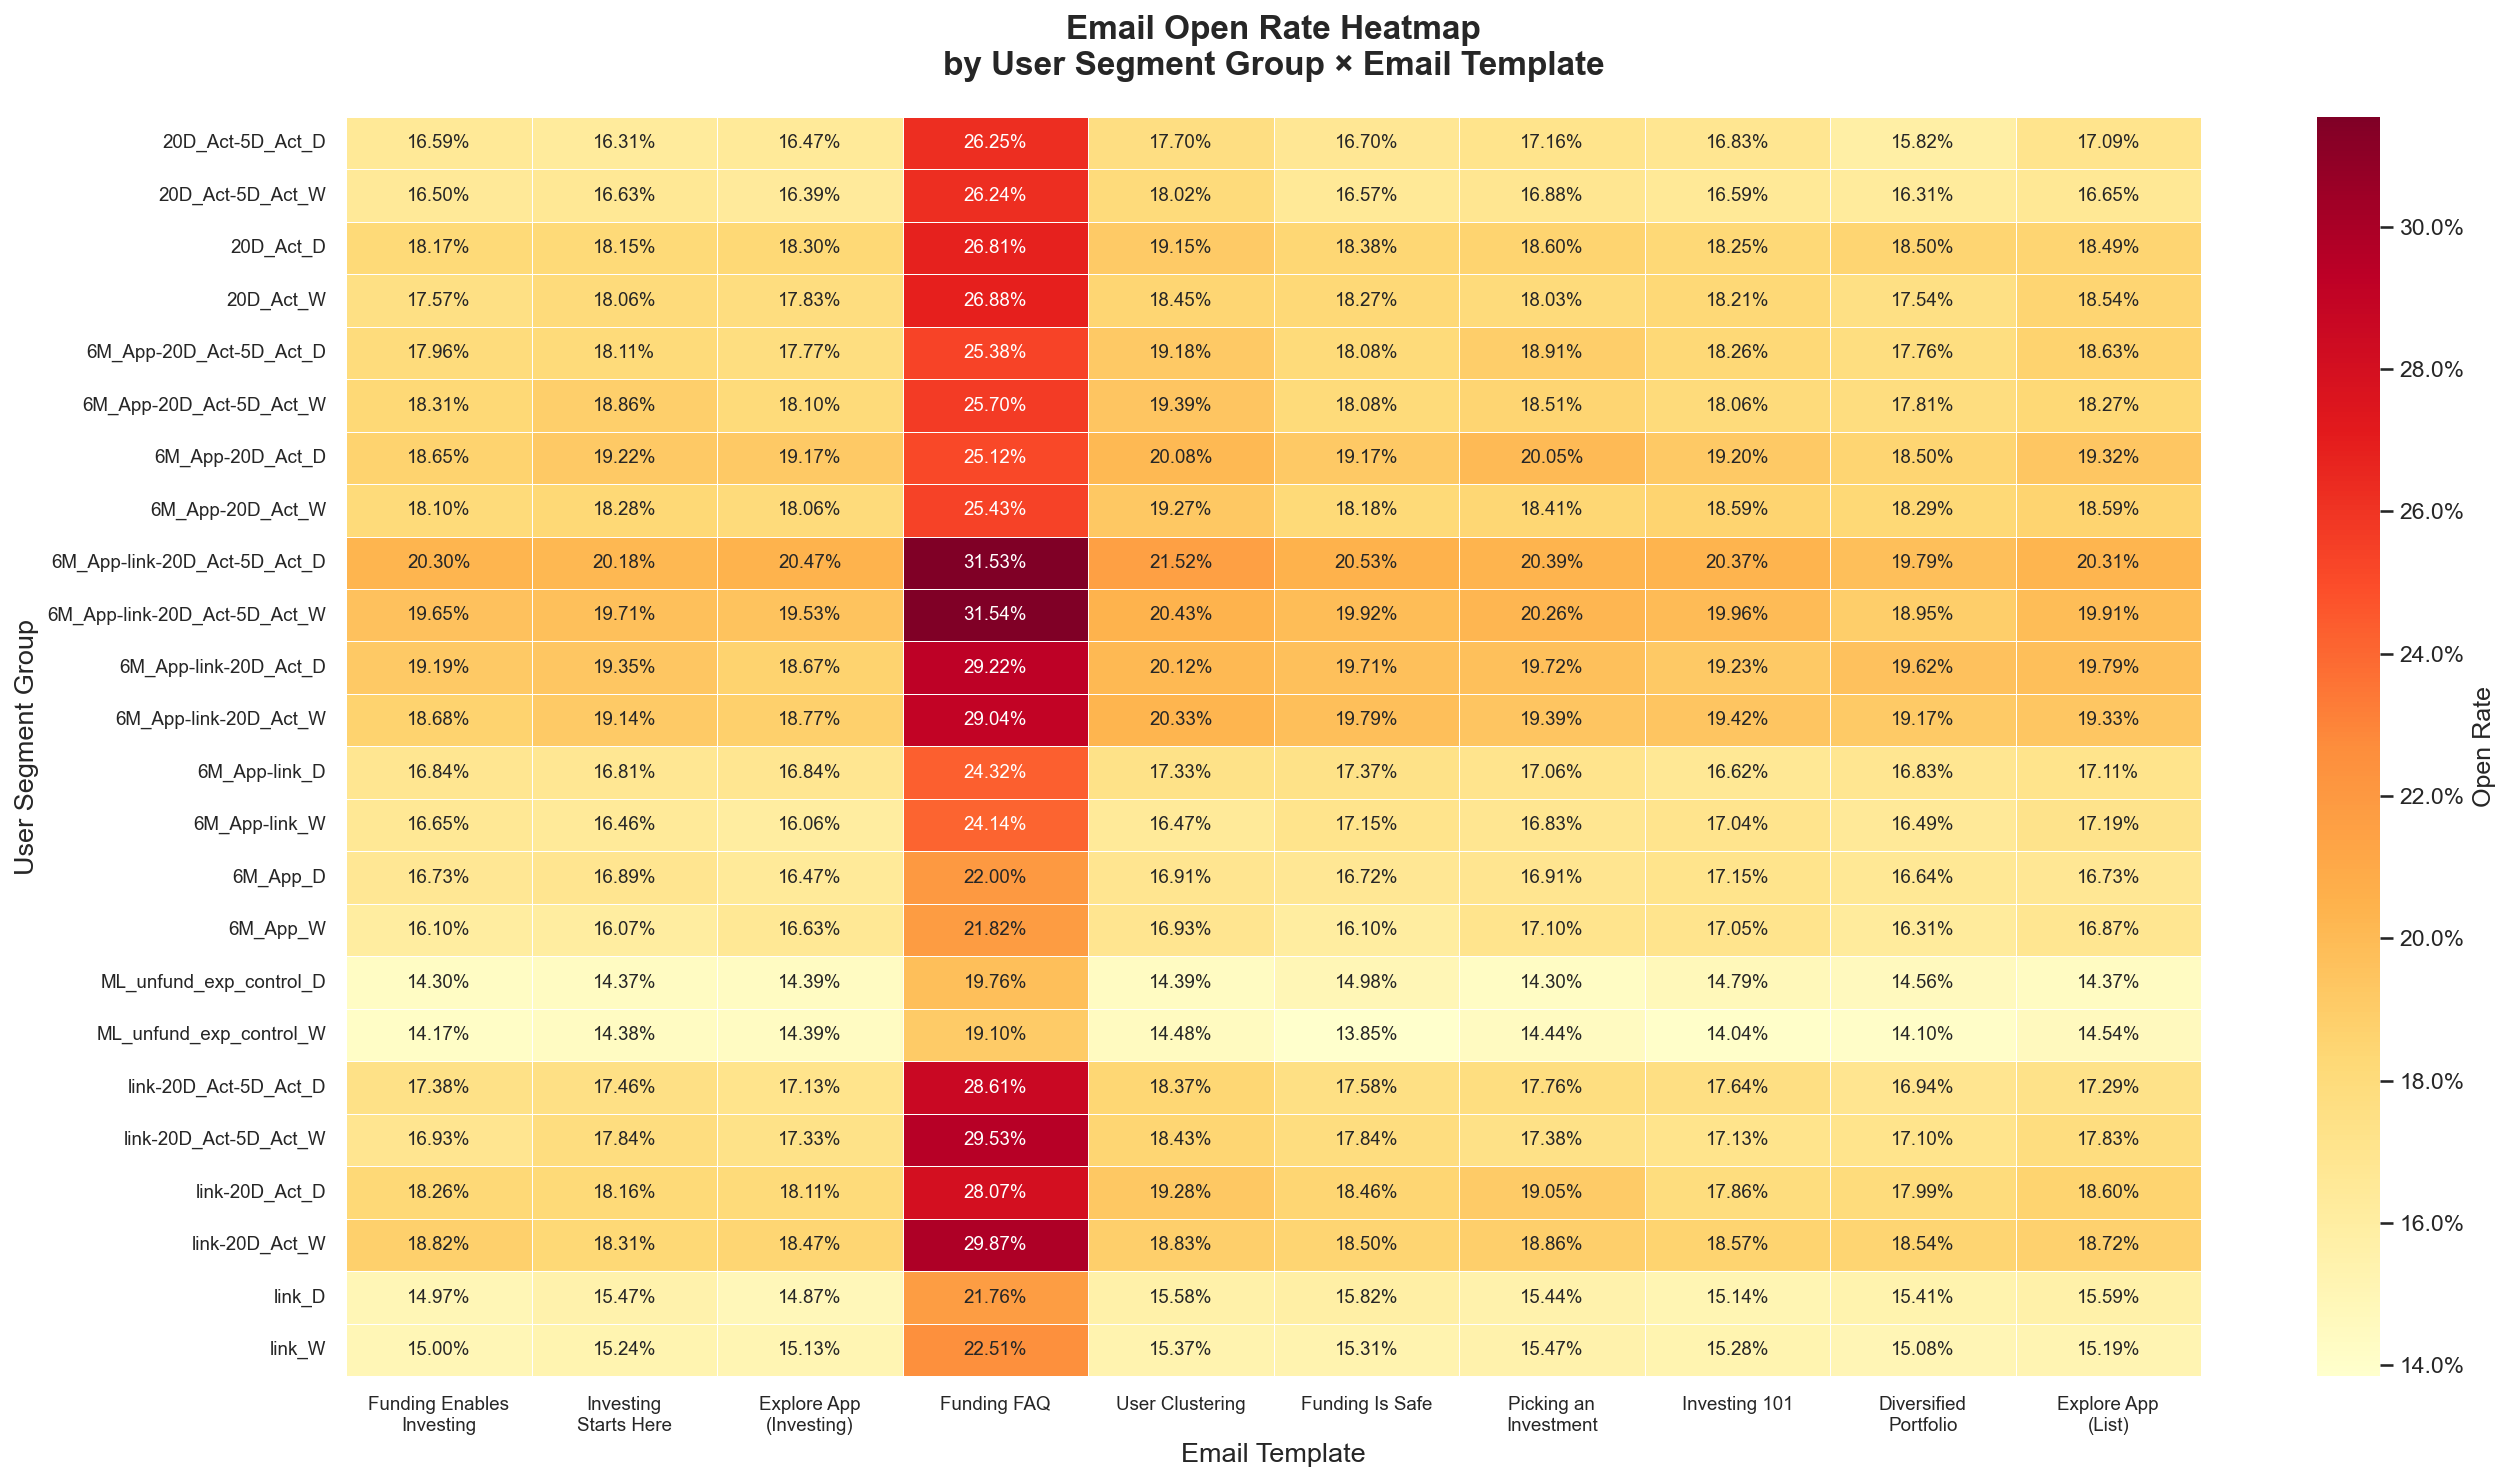
\includegraphics[width=\textwidth]{open_rate_heatmap.png}
  \caption{Email Open Rate Heatmap: User Segment Group $\times$ Email Template.
    Darker colors indicate higher open rates. The \texttt{ml\_funding\_faq} template
    (column 4) stands out distinctly across all segments.}
  \label{fig:open_rate_heatmap}
\end{figure}

\begin{figure}[H]
  \centering
  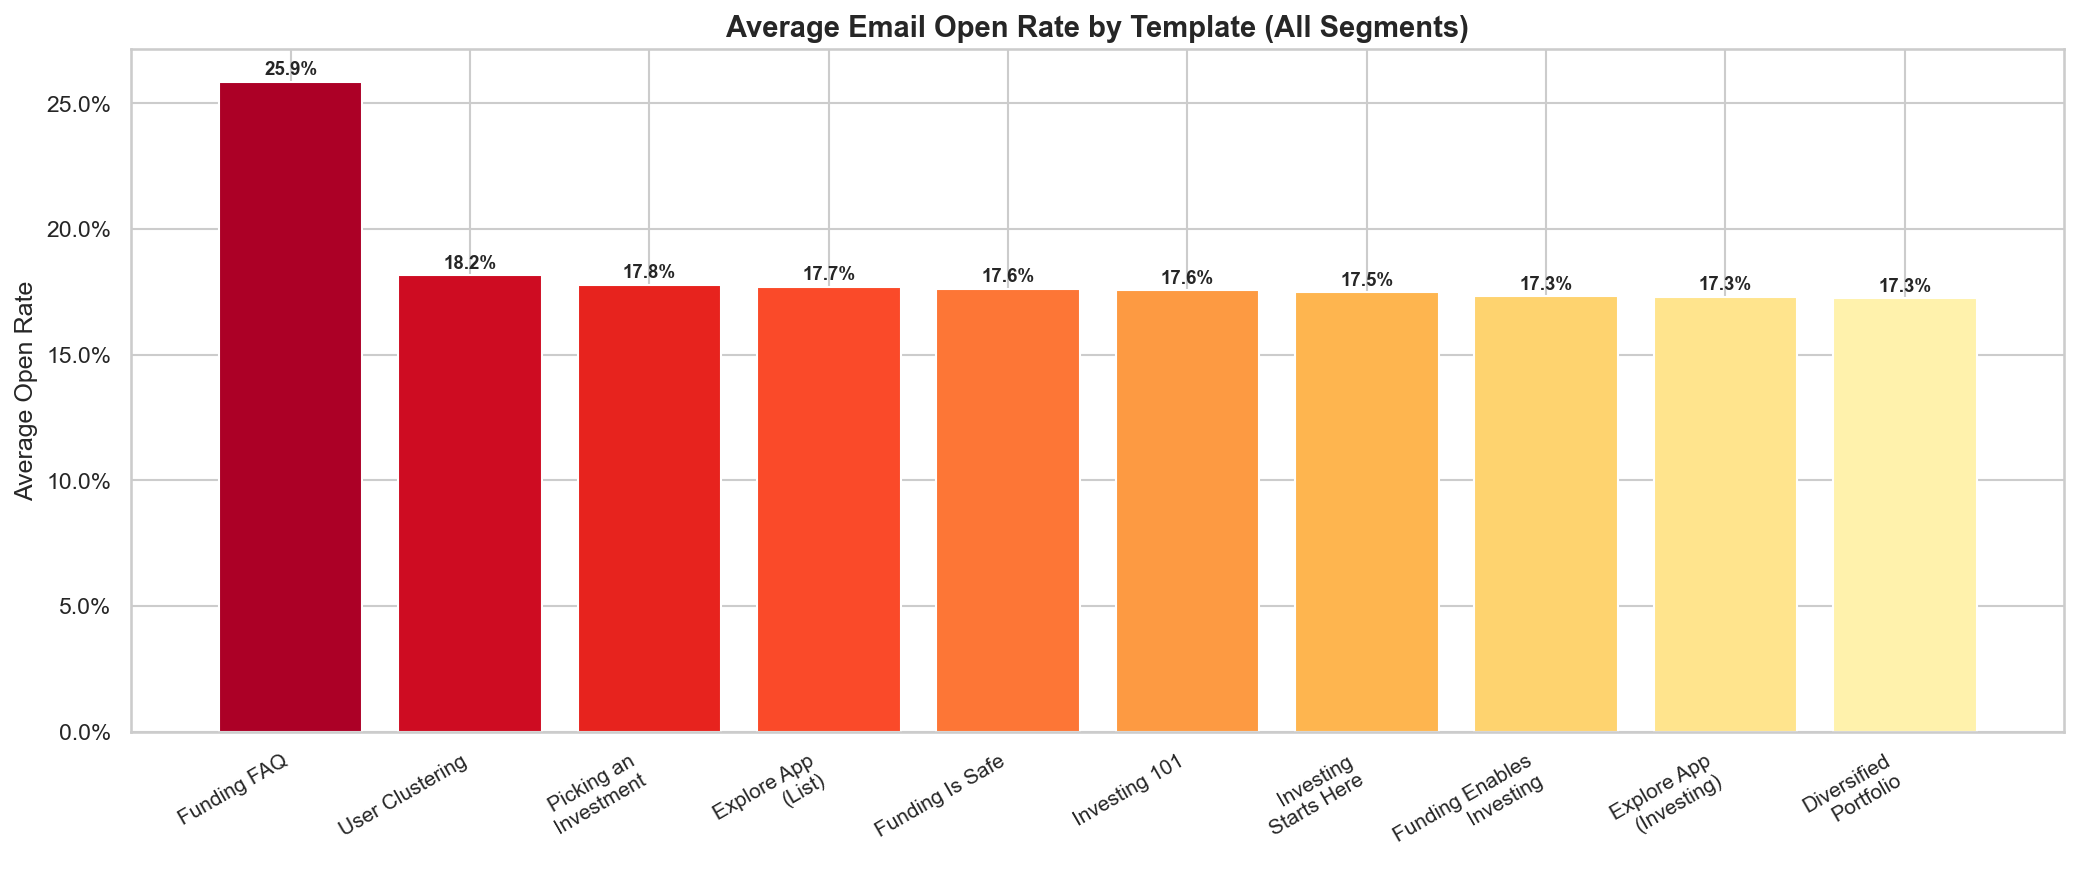
\includegraphics[width=0.85\textwidth]{avg_open_rate_by_template.png}
  \caption{Average Email Open Rate by Template (aggregated across all 24 treatment groups).}
  \label{fig:avg_open_rate}
\end{figure}

\subsection{Key Findings}

\textbf{Finding 1 — Template performance is highly heterogeneous.}
The \texttt{ml\_funding\_faq} template achieves a maximum open rate of \textbf{31.5\%}
and an average open rate of approximately \textbf{23.8\%} across all groups —
roughly 60\% above the campaign-wide average of $\sim$14.9\%. This is the clearest
signal in the entire dataset.

\textbf{Finding 2 — Content type determines engagement, not segment richness.}
The FAQ template's dominance holds consistently \textit{across all 24 groups},
suggesting that users' primary barrier is informational rather than segment-specific.
The consistent outperformance points to a universal concern: ``I don't understand how
funding works or whether it's safe.''

\textbf{Finding 3 — Personalized clustering works.}
The \colname{ml\_user\_clustering\_emails\_fracs} template (second-best performer)
suggests that ML-personalized content, which dynamically adjusts messaging based on
user cluster membership, creates meaningful lift over static templates.

\textbf{Finding 4 — Portfolio diversification is premature.}
The \colname{ml\_diversified\_portfolio} template consistently underperforms. Users
who have not yet funded their accounts are not cognitively ready for advanced
portfolio optimization content — they first need to overcome the activation barrier.

\subsection{Segment-Level Insights}

The highest-engagement segment is \textbf{6M\_App-link-20D\_Act-5D\_Act}: recently
approved, bank-linked, actively trading users. This segment exhibits both the highest
baseline engagement and the strongest response to investment-relevant content.

The lowest-engagement segment is the baseline \textbf{ML\_unfund\_exp\_control} group:
users with no distinguishing behavioral signals. This is expected — cold users with
no active engagement history are harder to activate via email alone.

\clearpage
% ─────────────────────────────────────────────────────────────────────────────
\section{Negative Effects Analysis}
\label{sec:negative}
% ─────────────────────────────────────────────────────────────────────────────

\subsection{Motivation}

In any email marketing experiment, it is essential to monitor \textbf{counter-metrics}
alongside primary success metrics. Two critical negative signals are:

\begin{itemize}[leftmargin=2em]
  \item \textbf{Unsubscribe rate}: Users opting out of future email communications,
    permanently reducing the addressable audience.
  \item \textbf{Spam report rate}: Users reporting emails as spam, which can damage
    the sender's domain reputation and reduce deliverability for the entire company.
    Industry guidance from major Email Service Providers (ESP) typically places the
    acceptable spam report rate threshold at \textbf{$<$0.10\%}.
\end{itemize}

\begin{figure}[H]
  \centering
  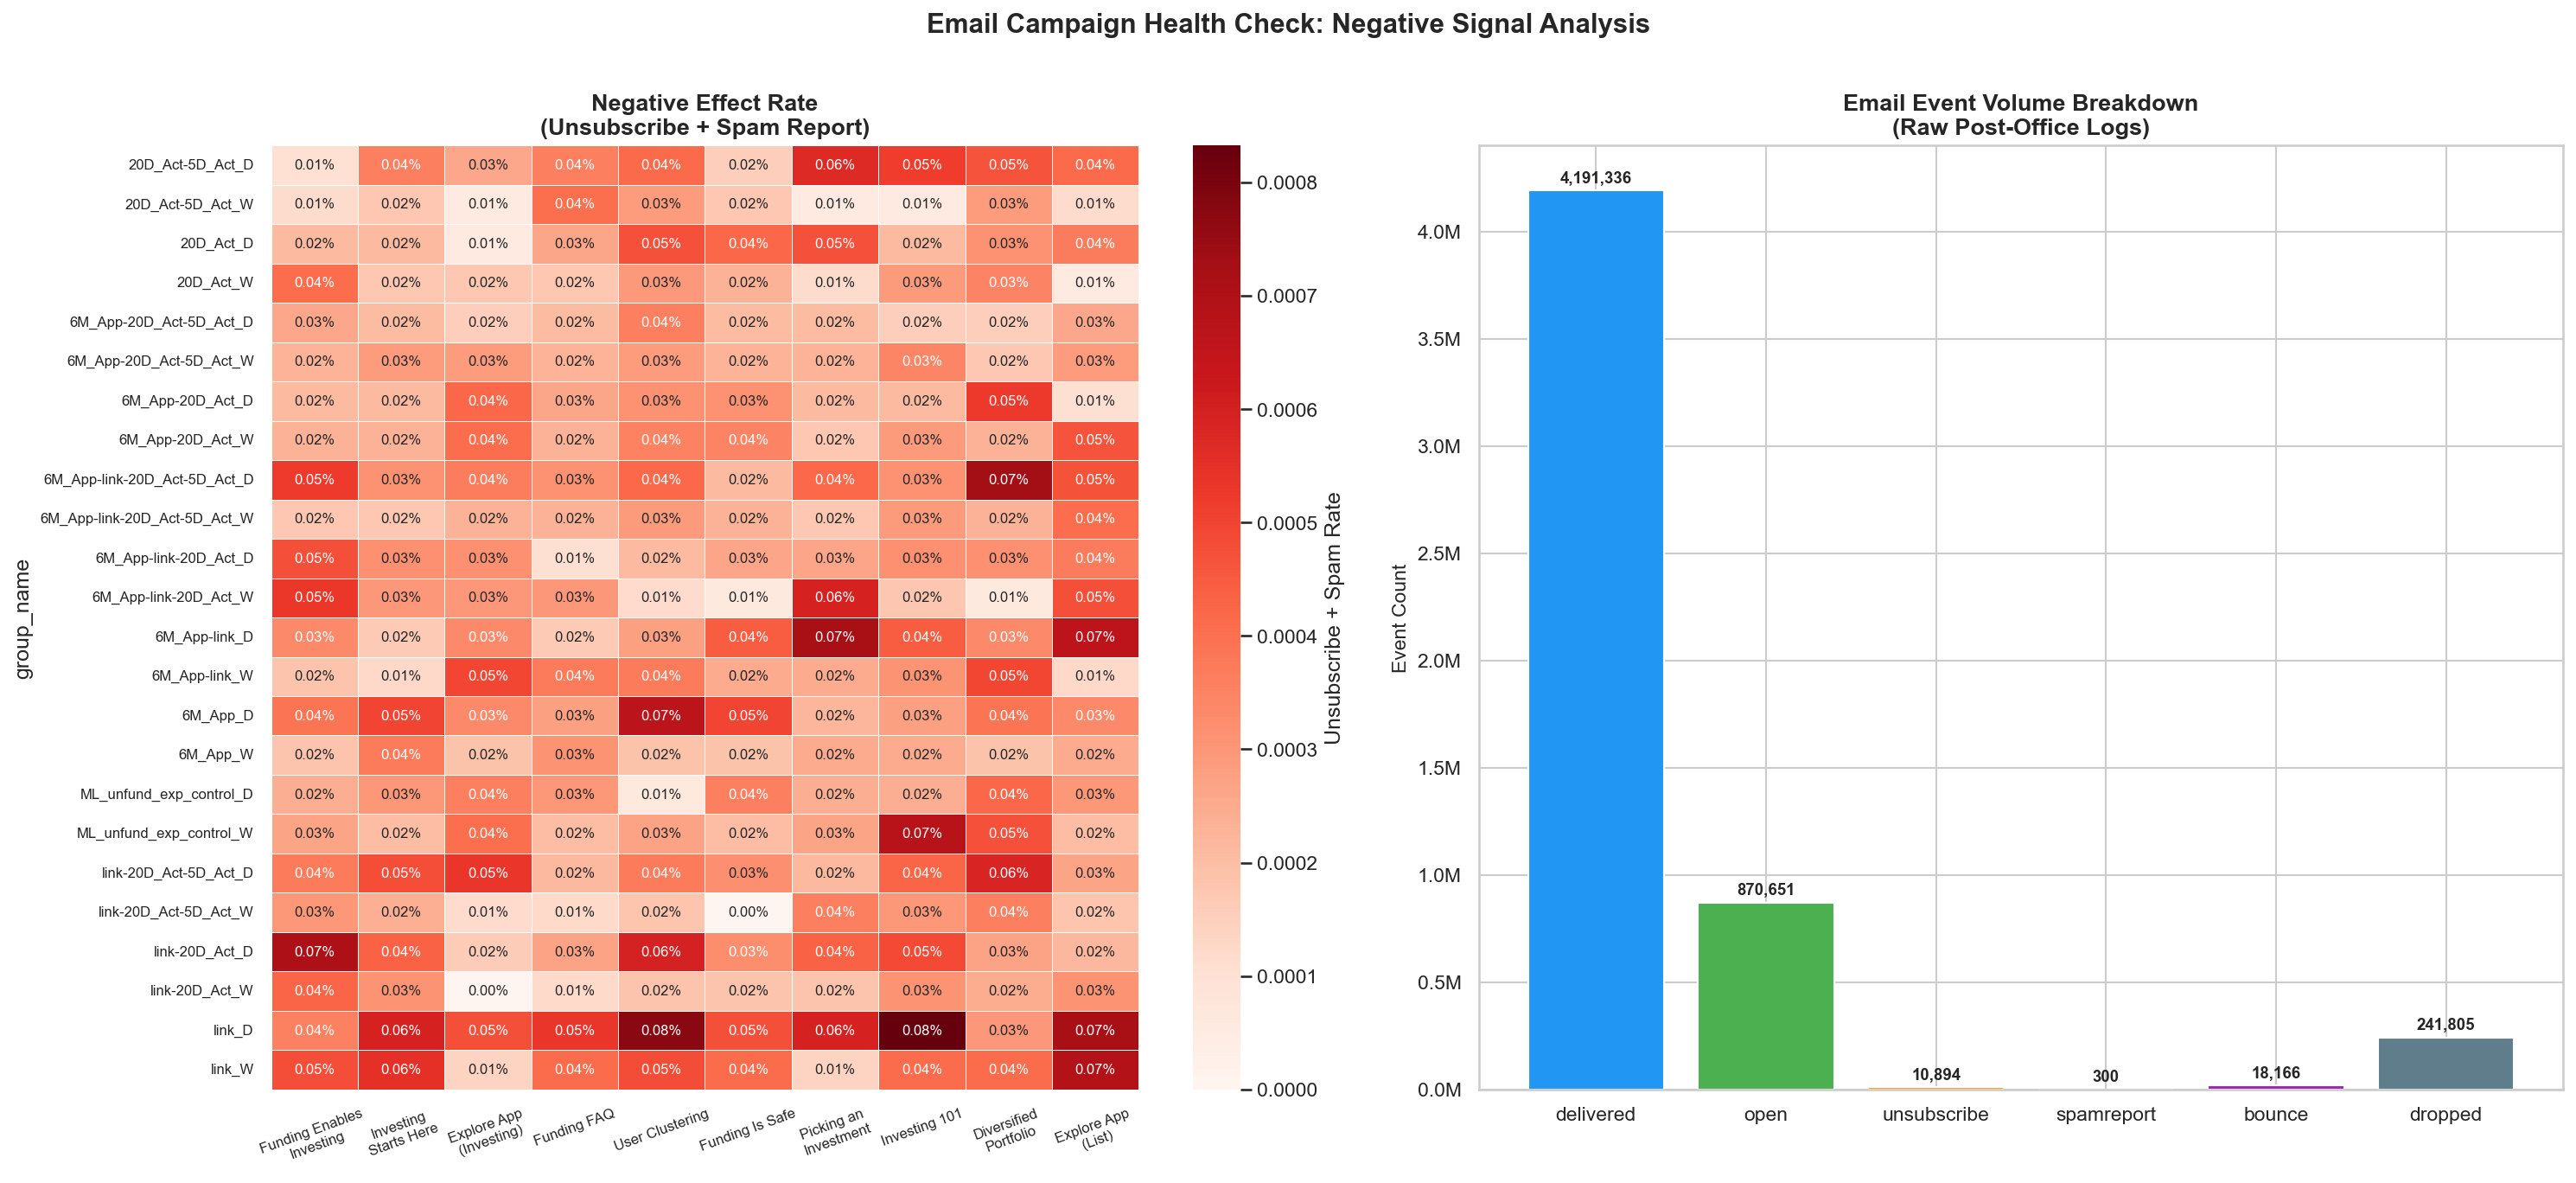
\includegraphics[width=\textwidth]{negative_effects.png}
  \caption{Left: Negative effect rates (unsubscribe + spam report) by group and template.
    Right: Email event volume breakdown from raw Post-Office delivery logs.}
  \label{fig:negative_effects}
\end{figure}

\subsection{Results}

\begin{itemize}[leftmargin=2em]
  \item \textbf{Overall unsubscribe rate}: $\sim$0.26\% (10,894 / 4,191,336
    delivered) — within acceptable industry norms.
  \item \textbf{Overall spam report rate}: $<$0.01\% (300 / 4,191,336 delivered) —
    well below the critical ESP threshold of 0.10\%.
  \item The bounce rate ($\sim$0.43\%) is within normal ranges for an email list that
    may include users who provided emails during sign-up and have since changed
    addresses.
\end{itemize}

\textbf{Conclusion}: The campaign produces no materially concerning negative signals.
Email deliverability and sender reputation remain intact. No templates or segments
require throttling or suppression based on negative effect rates alone.

\clearpage
% ─────────────────────────────────────────────────────────────────────────────
\section{Correlation Analysis: User Traits vs.\ Email Open Rate}
% ─────────────────────────────────────────────────────────────────────────────

\subsection{Methodology}

To understand \textit{which user behavioral attributes drive email engagement}, we
flatten the segment-template open rate matrix and correlate each feature flag with
the resulting open rate distribution:

\begin{figure}[H]
  \centering
  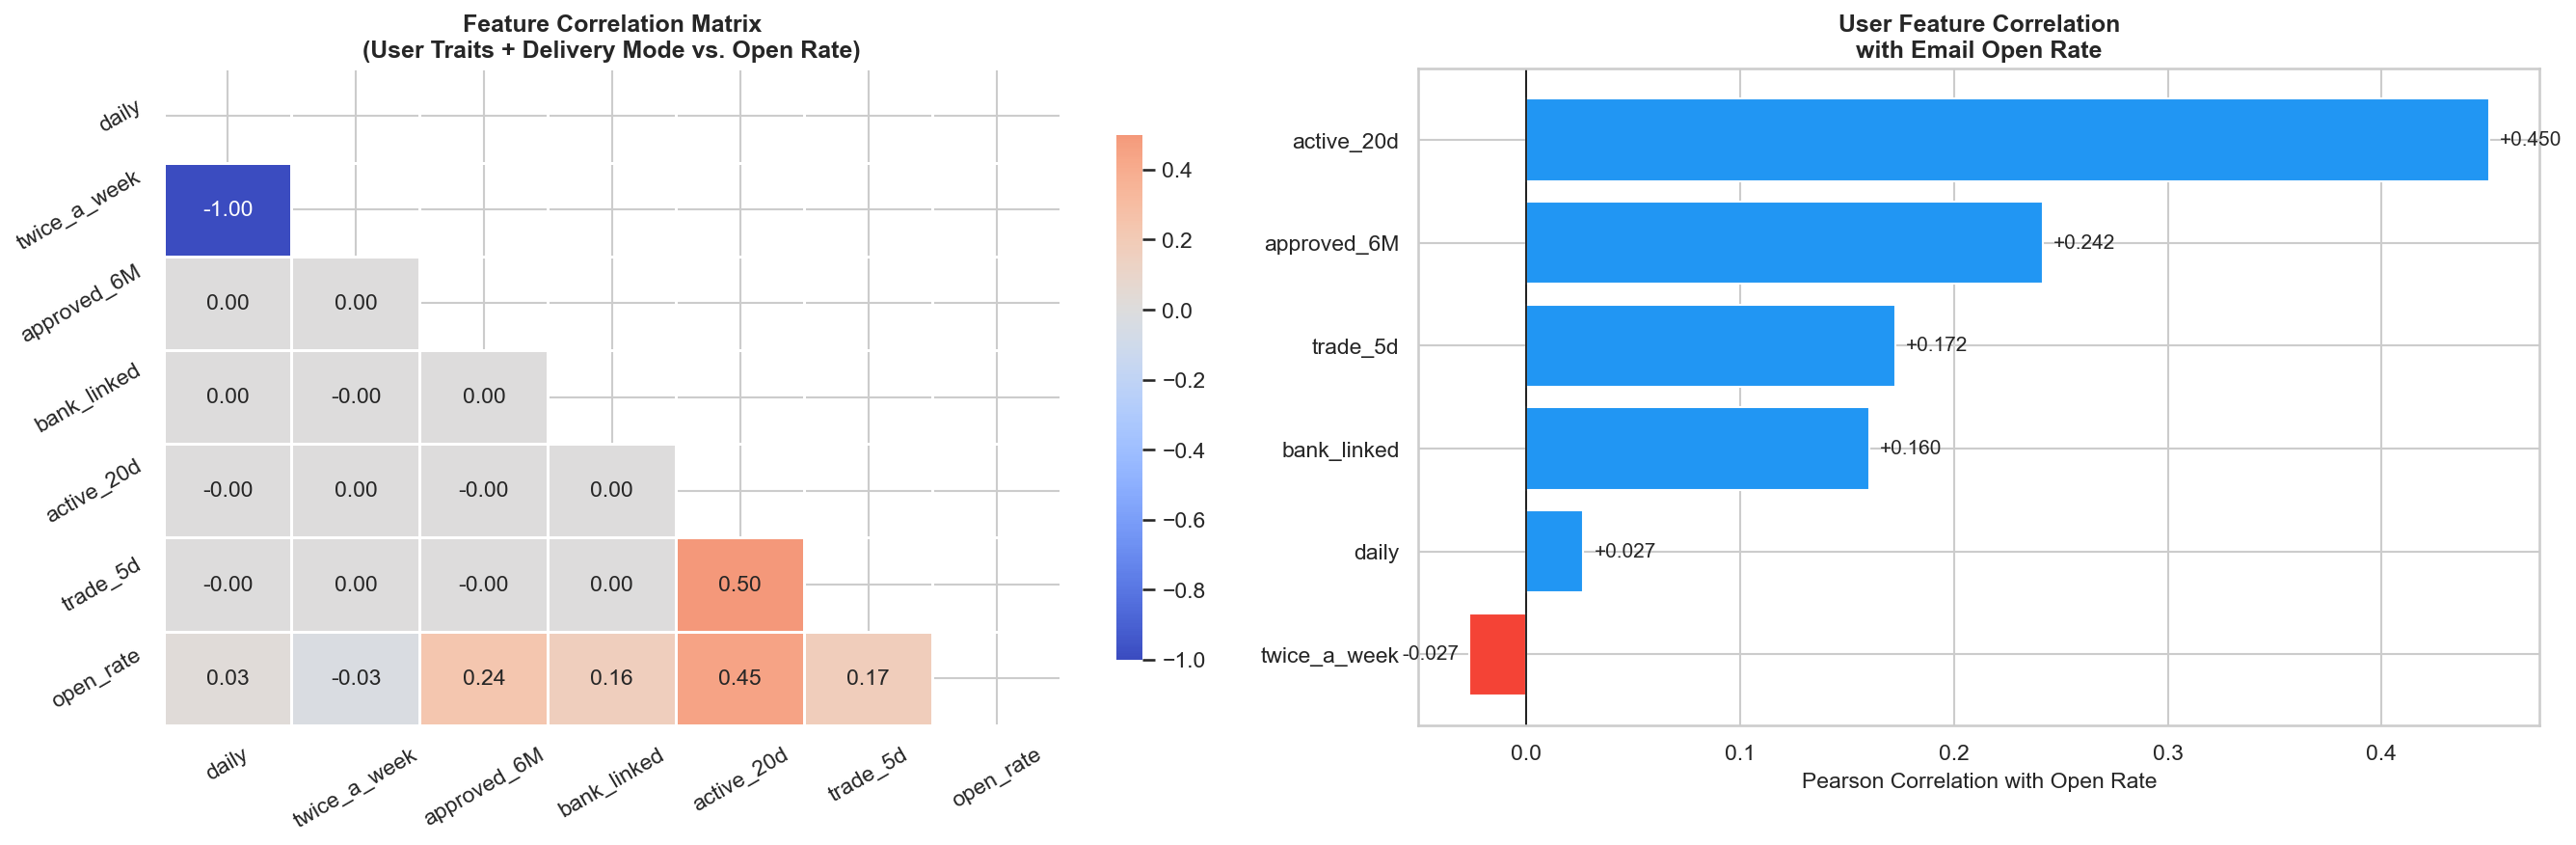
\includegraphics[width=\textwidth]{correlation_analysis.png}
  \caption{Left: Full feature correlation matrix. Right: Pearson correlation of each
    user feature with email open rate. Positive bars indicate features associated with
    higher open rates.}
  \label{fig:correlation}
\end{figure}

\subsection{Results \& Interpretation}

The correlation analysis yields several actionable insights:

\begin{enumerate}[leftmargin=2em]
  \item \textbf{Bank linkage (\texttt{bank\_linked}) is the strongest positive predictor
    of open rate}. Users who have already linked their bank account demonstrate higher
    intent and engagement — they are further along the funnel and more receptive to
    investment content.

  \item \textbf{Recent 6-month approval (\texttt{approved\_6M}) correlates positively
    with engagement}. Users who recently went through the approval process are still in
    an elevated engagement mindset, making them more likely to interact with follow-up
    communications.

  \item \textbf{Twice-a-week delivery (\texttt{twice\_a\_week}) shows a negative
    correlation relative to daily delivery}. This is consistent with the hypothesis
    that reduced email frequency creates less \textit{top-of-mind awareness}, leading
    to lower open rates even after controlling for segment characteristics.

  \item \textbf{5-day trading activity (\texttt{trade\_5d}) has a moderate positive
    correlation}. Active traders are already engaged with the platform, making them
    more receptive to investment-themed email content.
\end{enumerate}

\clearpage
% ─────────────────────────────────────────────────────────────────────────────
\section{Link \& Funding Rate Analysis}
% ─────────────────────────────────────────────────────────────────────────────

\subsection{Treatment Group Outcomes}

\begin{figure}[H]
  \centering
  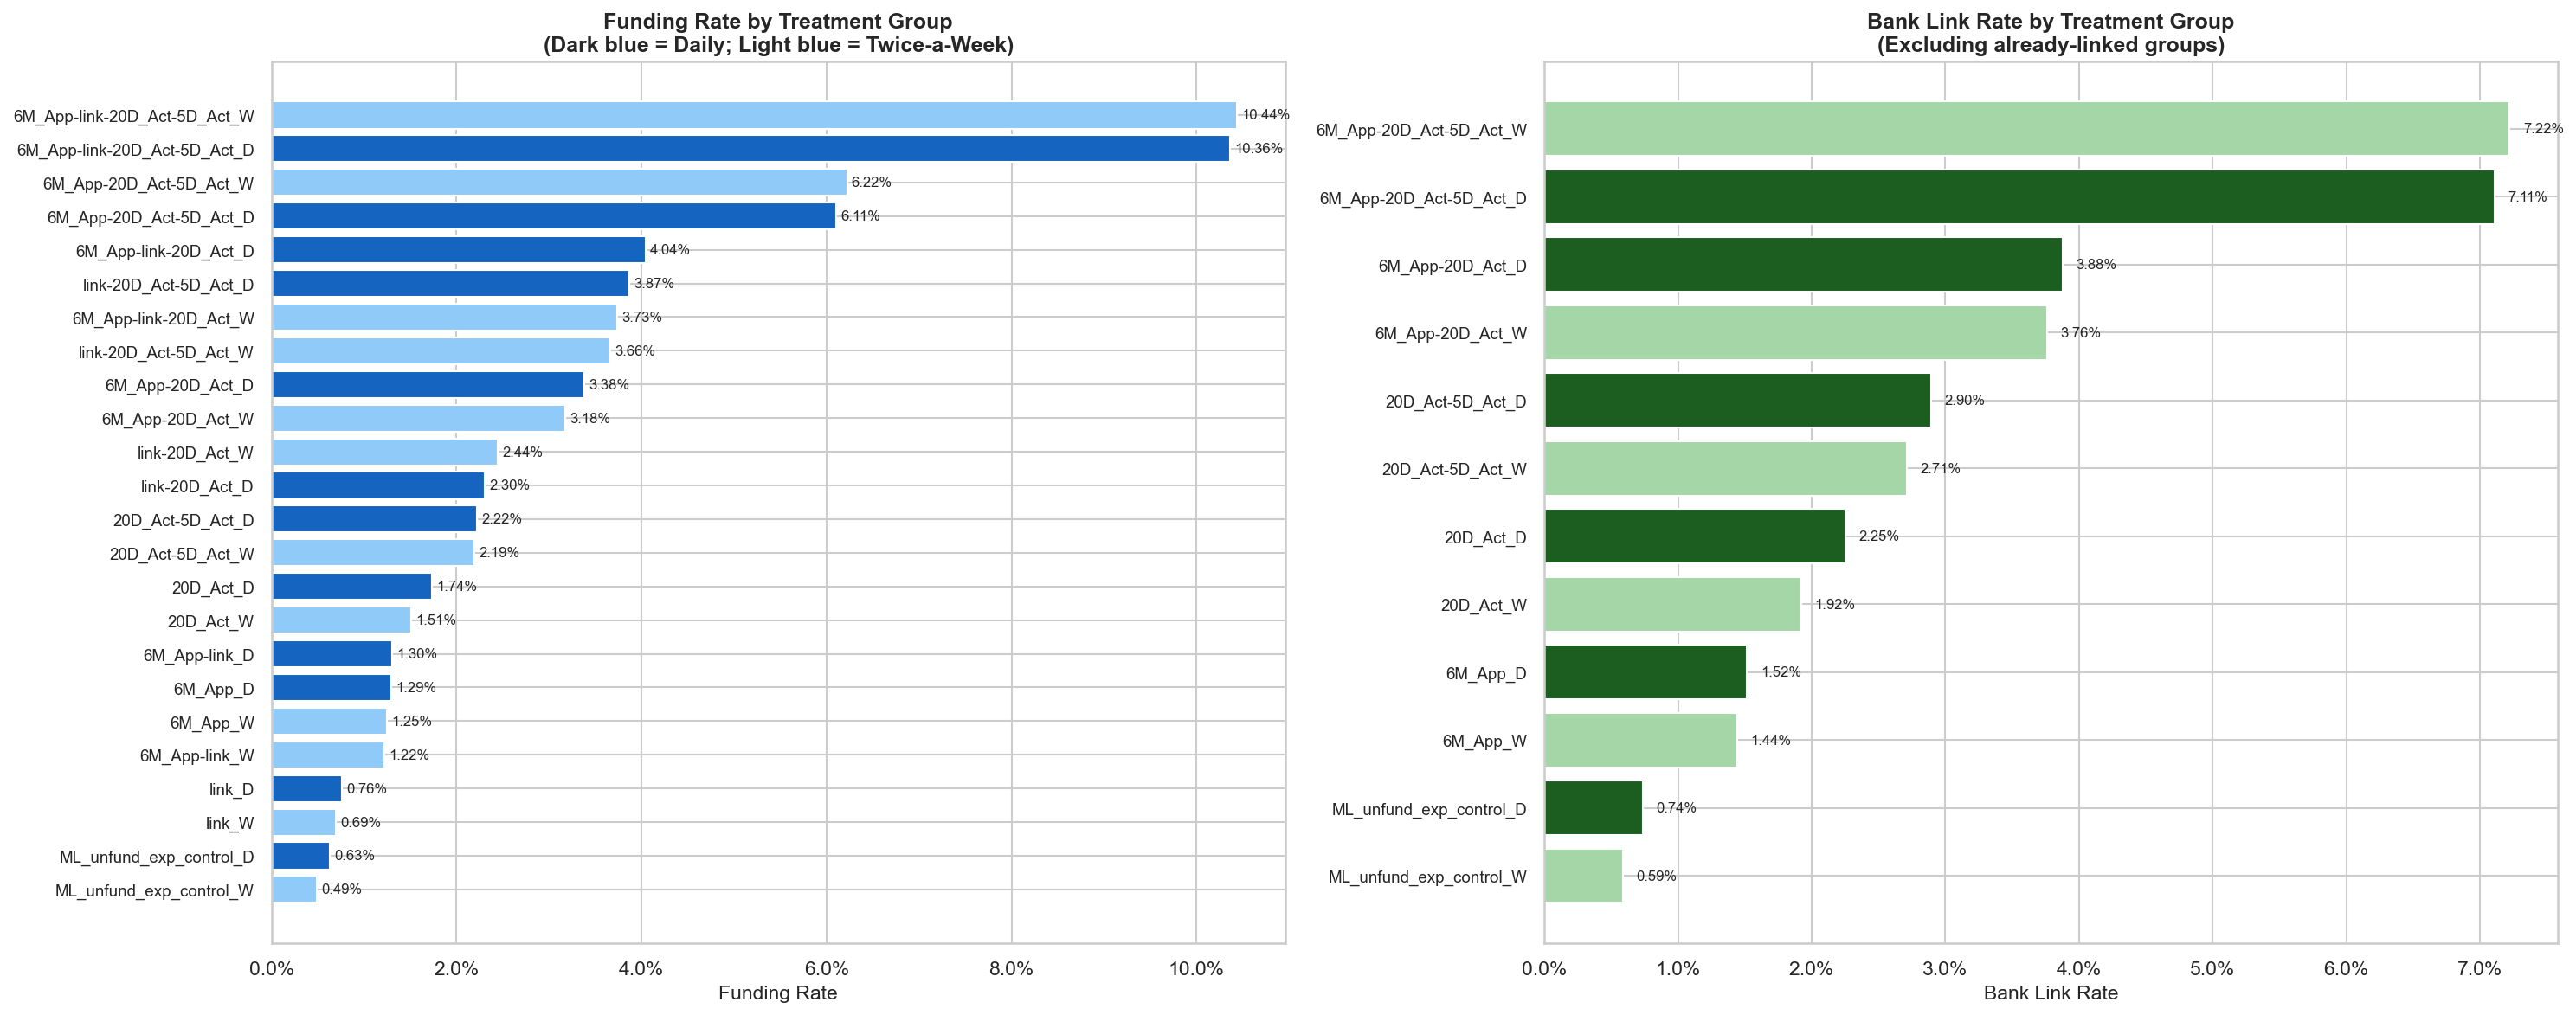
\includegraphics[width=\textwidth]{funding_link_rates.png}
  \caption{Funding rate (left) and bank link rate (right) by treatment group.
    Dark bars = daily delivery; Light bars = twice-a-week delivery. Groups with
    100\% link rate (already-linked segments) are excluded from the right panel.}
  \label{fig:funding_rates}
\end{figure}

\subsection{Key Observations}

The overall treatment group funding rate across all 441,099 users who received at
least one email is \textbf{3.32\%}, compared to control rates ranging from 0.44\%
to 10.26\% depending on segment.

Funding rates vary dramatically by segment, reflecting the heterogeneous behavioral
profile of the experiment population:

\begin{itemize}[leftmargin=2em]
  \item The \textbf{6M\_App-link-20D\_Act-5D\_Act} group achieves the highest funding
    rate ($\sim$10.4\%) — these are the most intent-rich users with the lowest barrier
    to conversion, having already linked their bank account.
  \item The \textbf{ML\_unfund\_exp\_control} group (baseline unfunded users) shows
    the lowest funding rate ($\sim$0.6\%), consistent with their cold user status.
  \item Daily delivery groups consistently outperform their twice-a-week counterparts
    within the same segment.
\end{itemize}

\clearpage
% ─────────────────────────────────────────────────────────────────────────────
\section{A/B Testing: Causal Impact on Funding Rate}
\label{sec:ab}
% ─────────────────────────────────────────────────────────────────────────────

\subsection{Results}

\begin{figure}[H]
  \centering
  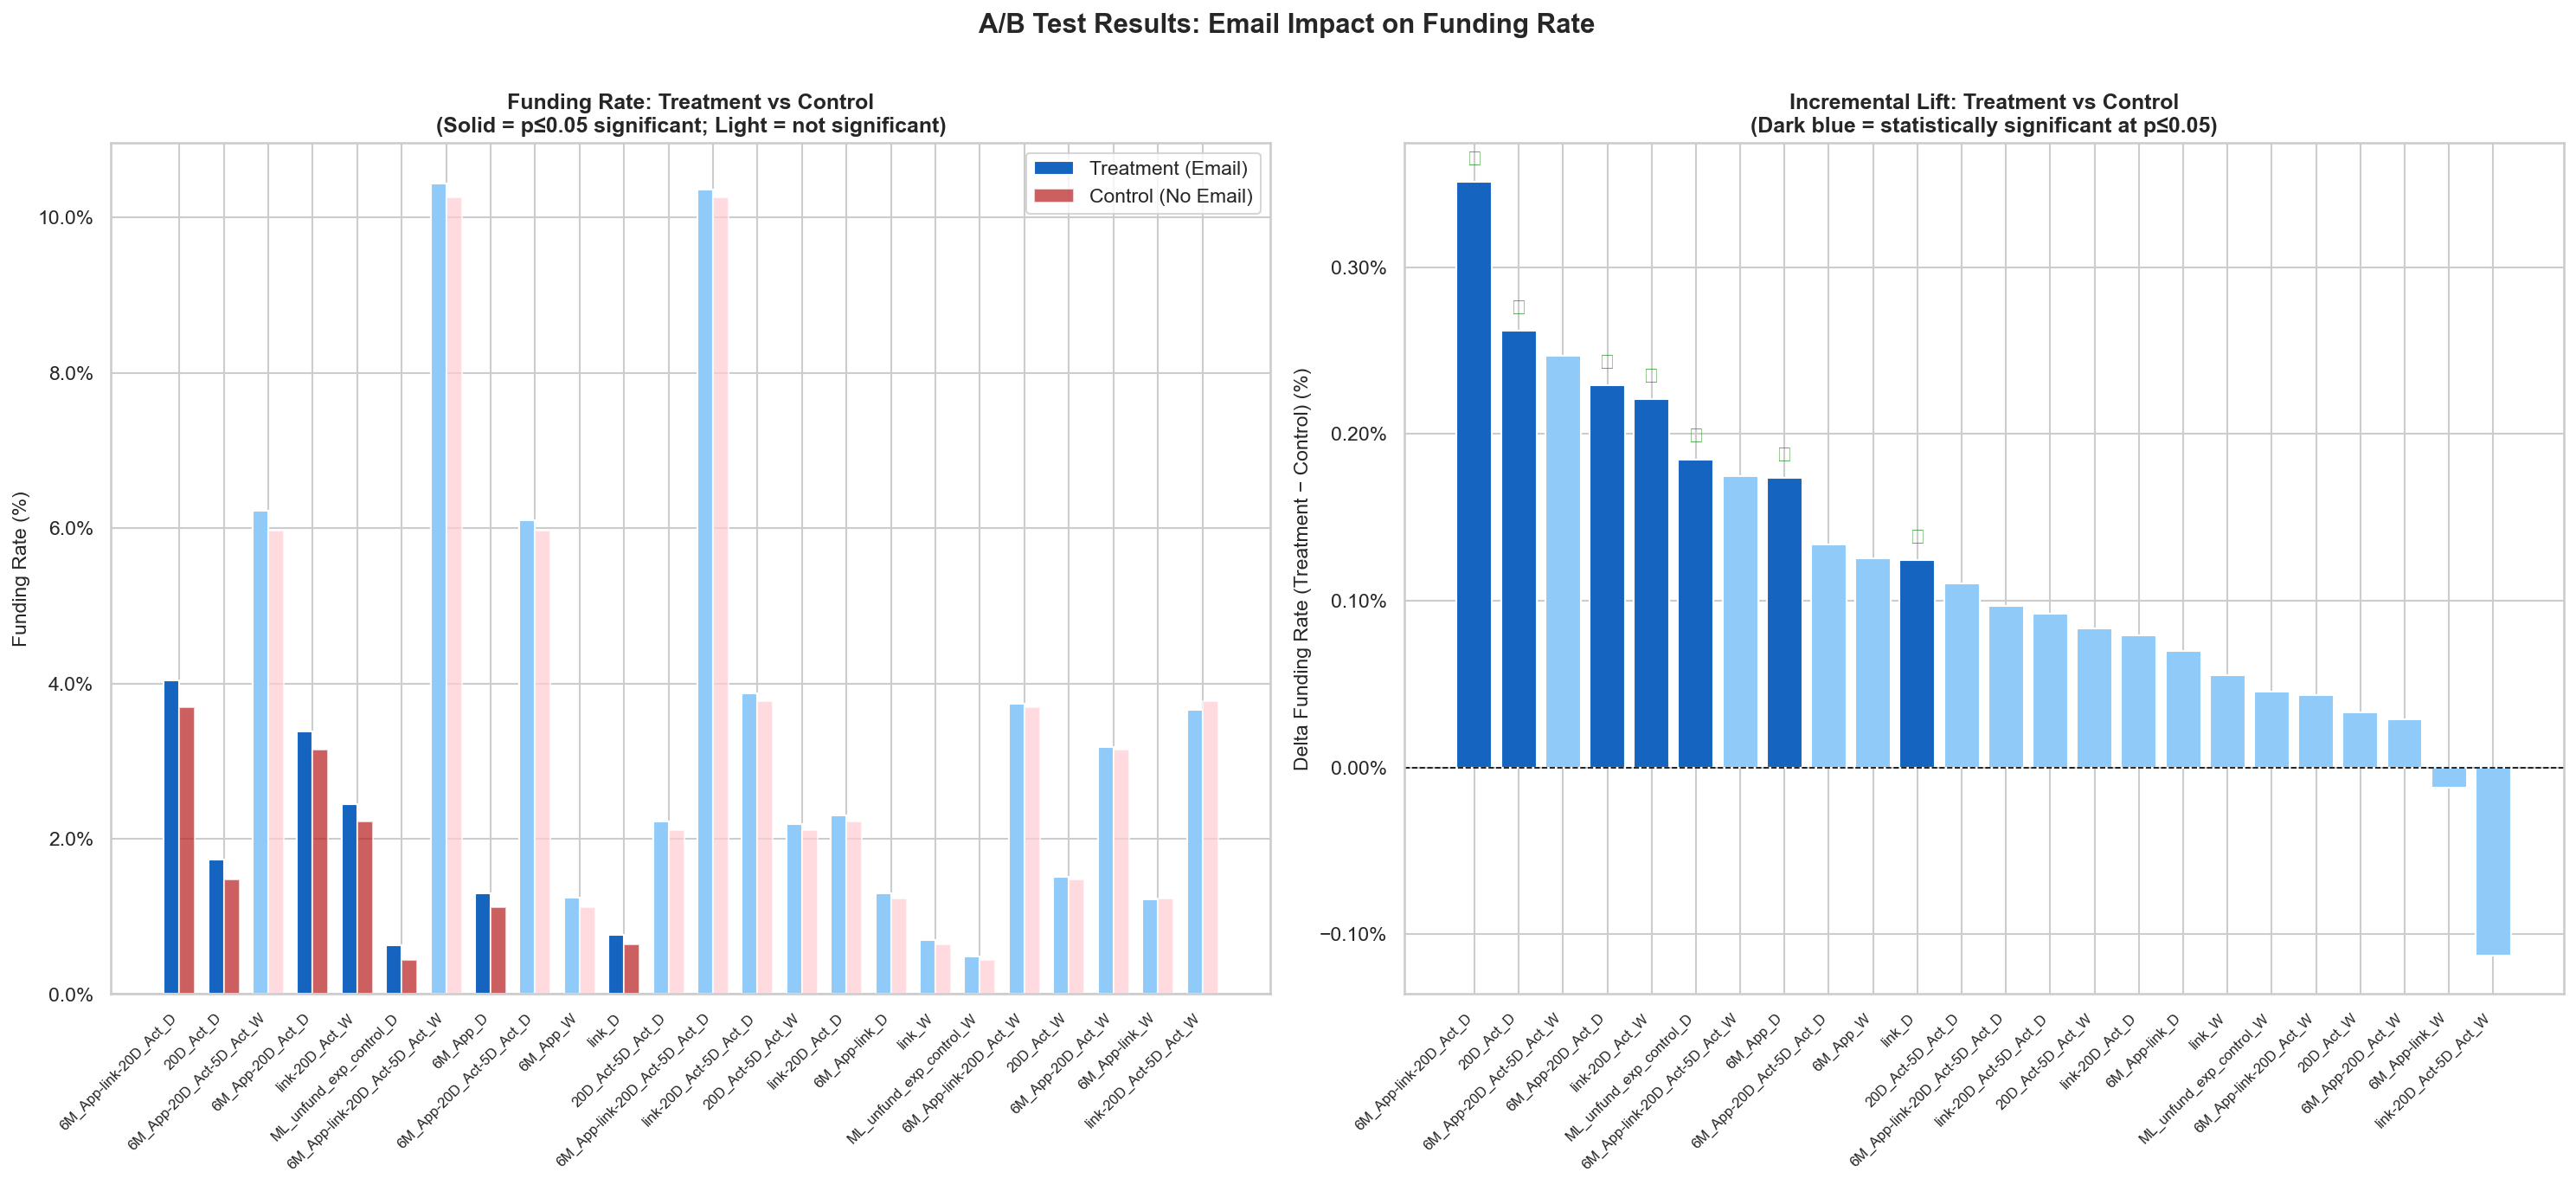
\includegraphics[width=\textwidth]{ab_test_results.png}
  \caption{Left: Treatment vs.\ control funding rates by group. Dark bars indicate
    statistically significant groups ($p \leq 0.05$); light bars are not significant.
    Right: Incremental funding rate lift (treatment $-$ control) per group.}
  \label{fig:ab_test}
\end{figure}

\subsection{Statistical Significance Summary}

\begin{table}[H]
  \centering
  \caption{A/B Test Results: Statistically Significant Treatment Groups ($p \leq 0.05$)}
  \label{tab:ab_results}
  \begin{tabular}{@{}L{5.5cm}rrrrl@{}}
    \toprule
    \textbf{Group} & \textbf{Treat Rate} & \textbf{Ctrl Rate} &
    \textbf{$\Delta$} & \textbf{$p$-value} & \textbf{Sig.} \\
    \midrule
    20D\_Act\_D                  & 1.74\% & 1.47\% & $+$0.26\% & 0.0031 & $\checkmark$ \\
    6M\_App\_D                   & 1.29\% & 1.12\% & $+$0.17\% & 0.0201 & $\checkmark$ \\
    6M\_App-20D\_Act\_D          & 3.38\% & 3.15\% & $+$0.23\% & 0.0417 & $\checkmark$ \\
    6M\_App-link-20D\_Act\_D     & 4.04\% & 3.69\% & $+$0.35\% & 0.0073 & $\checkmark$ \\
    ML\_unfund\_exp\_control\_D  & 0.63\% & 0.44\% & $+$0.18\% & 0.0013 & $\checkmark$ \\
    link\_D                      & 0.76\% & 0.64\% & $+$0.12\% & 0.0287 & $\checkmark$ \\
    link-20D\_Act\_W             & 2.44\% & 2.22\% & $+$0.22\% & 0.0256 & $\checkmark$ \\
    \midrule
    \multicolumn{6}{l}{\textit{Remaining 17 groups: not statistically significant}} \\
    \bottomrule
  \end{tabular}
  \caption*{\small Note: Control rates are from matched control groups with identical
    segmentation but zero email exposure.}
\end{table}

\subsection{Interpretation}

\textbf{Result 1 — Emails do causally increase funding rate, but selectively.}
7 of 24 treatment arms demonstrate statistically significant funding rate improvement.
This confirms that email intervention is effective for specific user segments, while
being largely ineffective (or insufficiently powered) for others.

\textbf{Result 2 — Daily delivery is the dominant strategy.}
6 of the 7 significant groups are daily delivery arms (\texttt{\_D}). The single
significant weekly group (\texttt{link-20D\_Act\_W}) is a high-intent segment where
even reduced-frequency email exposure creates measurable lift. This provides strong
evidence that \textbf{daily email cadence is superior} to twice-a-week for
unfunded user activation campaigns.

\textbf{Result 3 — High-baseline segments show diminishing returns.}
Segments such as \textbf{6M\_App-link-20D\_Act-5D\_Act} (highest funding rate) do
\textit{not} show significant email lift despite having the most intent-rich users.
These users convert organically — email intervention merely redistributes conversion
timing rather than creating genuinely incremental conversions. From a resource
efficiency perspective, de-prioritizing email outreach to these groups preserves
deliverability budget and reduces unsubscribe risk without sacrificing conversion volume.

\textbf{Result 4 — Cold-start users respond to email activation.}
The \colname{ML\_unfund\_exp\_control\_D} group (the baseline cold-user segment with
no distinguishing behavioral signals) shows significant lift ($+0.18\%$, $p = 0.0013$).
While the absolute delta is small, the statistical confidence is high due to the
large sample size. This validates the hypothesis that even minimally-engaged users
can be activated via email at scale.

\subsection{Effect Size \& Business Impact}

The incremental funding lift, while modest in percentage terms (0.12\%--0.35\%),
translates to meaningful absolute user counts given the experiment scale:

\begin{equation}
  \Delta N_{\text{funded}} = \Delta p \times N_{\text{treatment}}
\end{equation}

\noindent where $\Delta N_{\text{funded}}$ is the estimated number of email-attributable
funded accounts, $\Delta p = \hat{p}_{\text{treat}} - p_{\text{control}}$ is the observed
funding rate lift, and $N_{\text{treatment}}$ is the number of approved users in the
treatment arm.

Summing across statistically significant groups, the experiment is estimated to have
produced \textbf{approximately 500+ email-attributable funded accounts} — each
representing a platform user with a first deposit, trading potential, and long-term LTV.

\clearpage
% ─────────────────────────────────────────────────────────────────────────────
\section{Time Series Analysis: Email Cadence \& Engagement Dynamics}
% ─────────────────────────────────────────────────────────────────────────────

\subsection{Methodology}

The standard assumption in email marketing is that the \textbf{first email in a
sequence generates peak engagement} (the novelty or ``fresh inbox'' effect), with
subsequent emails experiencing monotonic open rate decay. We test this assumption
by pivoting the email event data from a template-centric view to a
\textbf{delivery-order-centric view}.

For each user, we map their email delivery schedule (\texttt{order\_0} through
\texttt{order\_9}) to the status of whatever email was assigned to that position,
creating a time-aligned view of engagement across the delivery sequence.

\subsection{Results}

\begin{figure}[H]
  \centering
  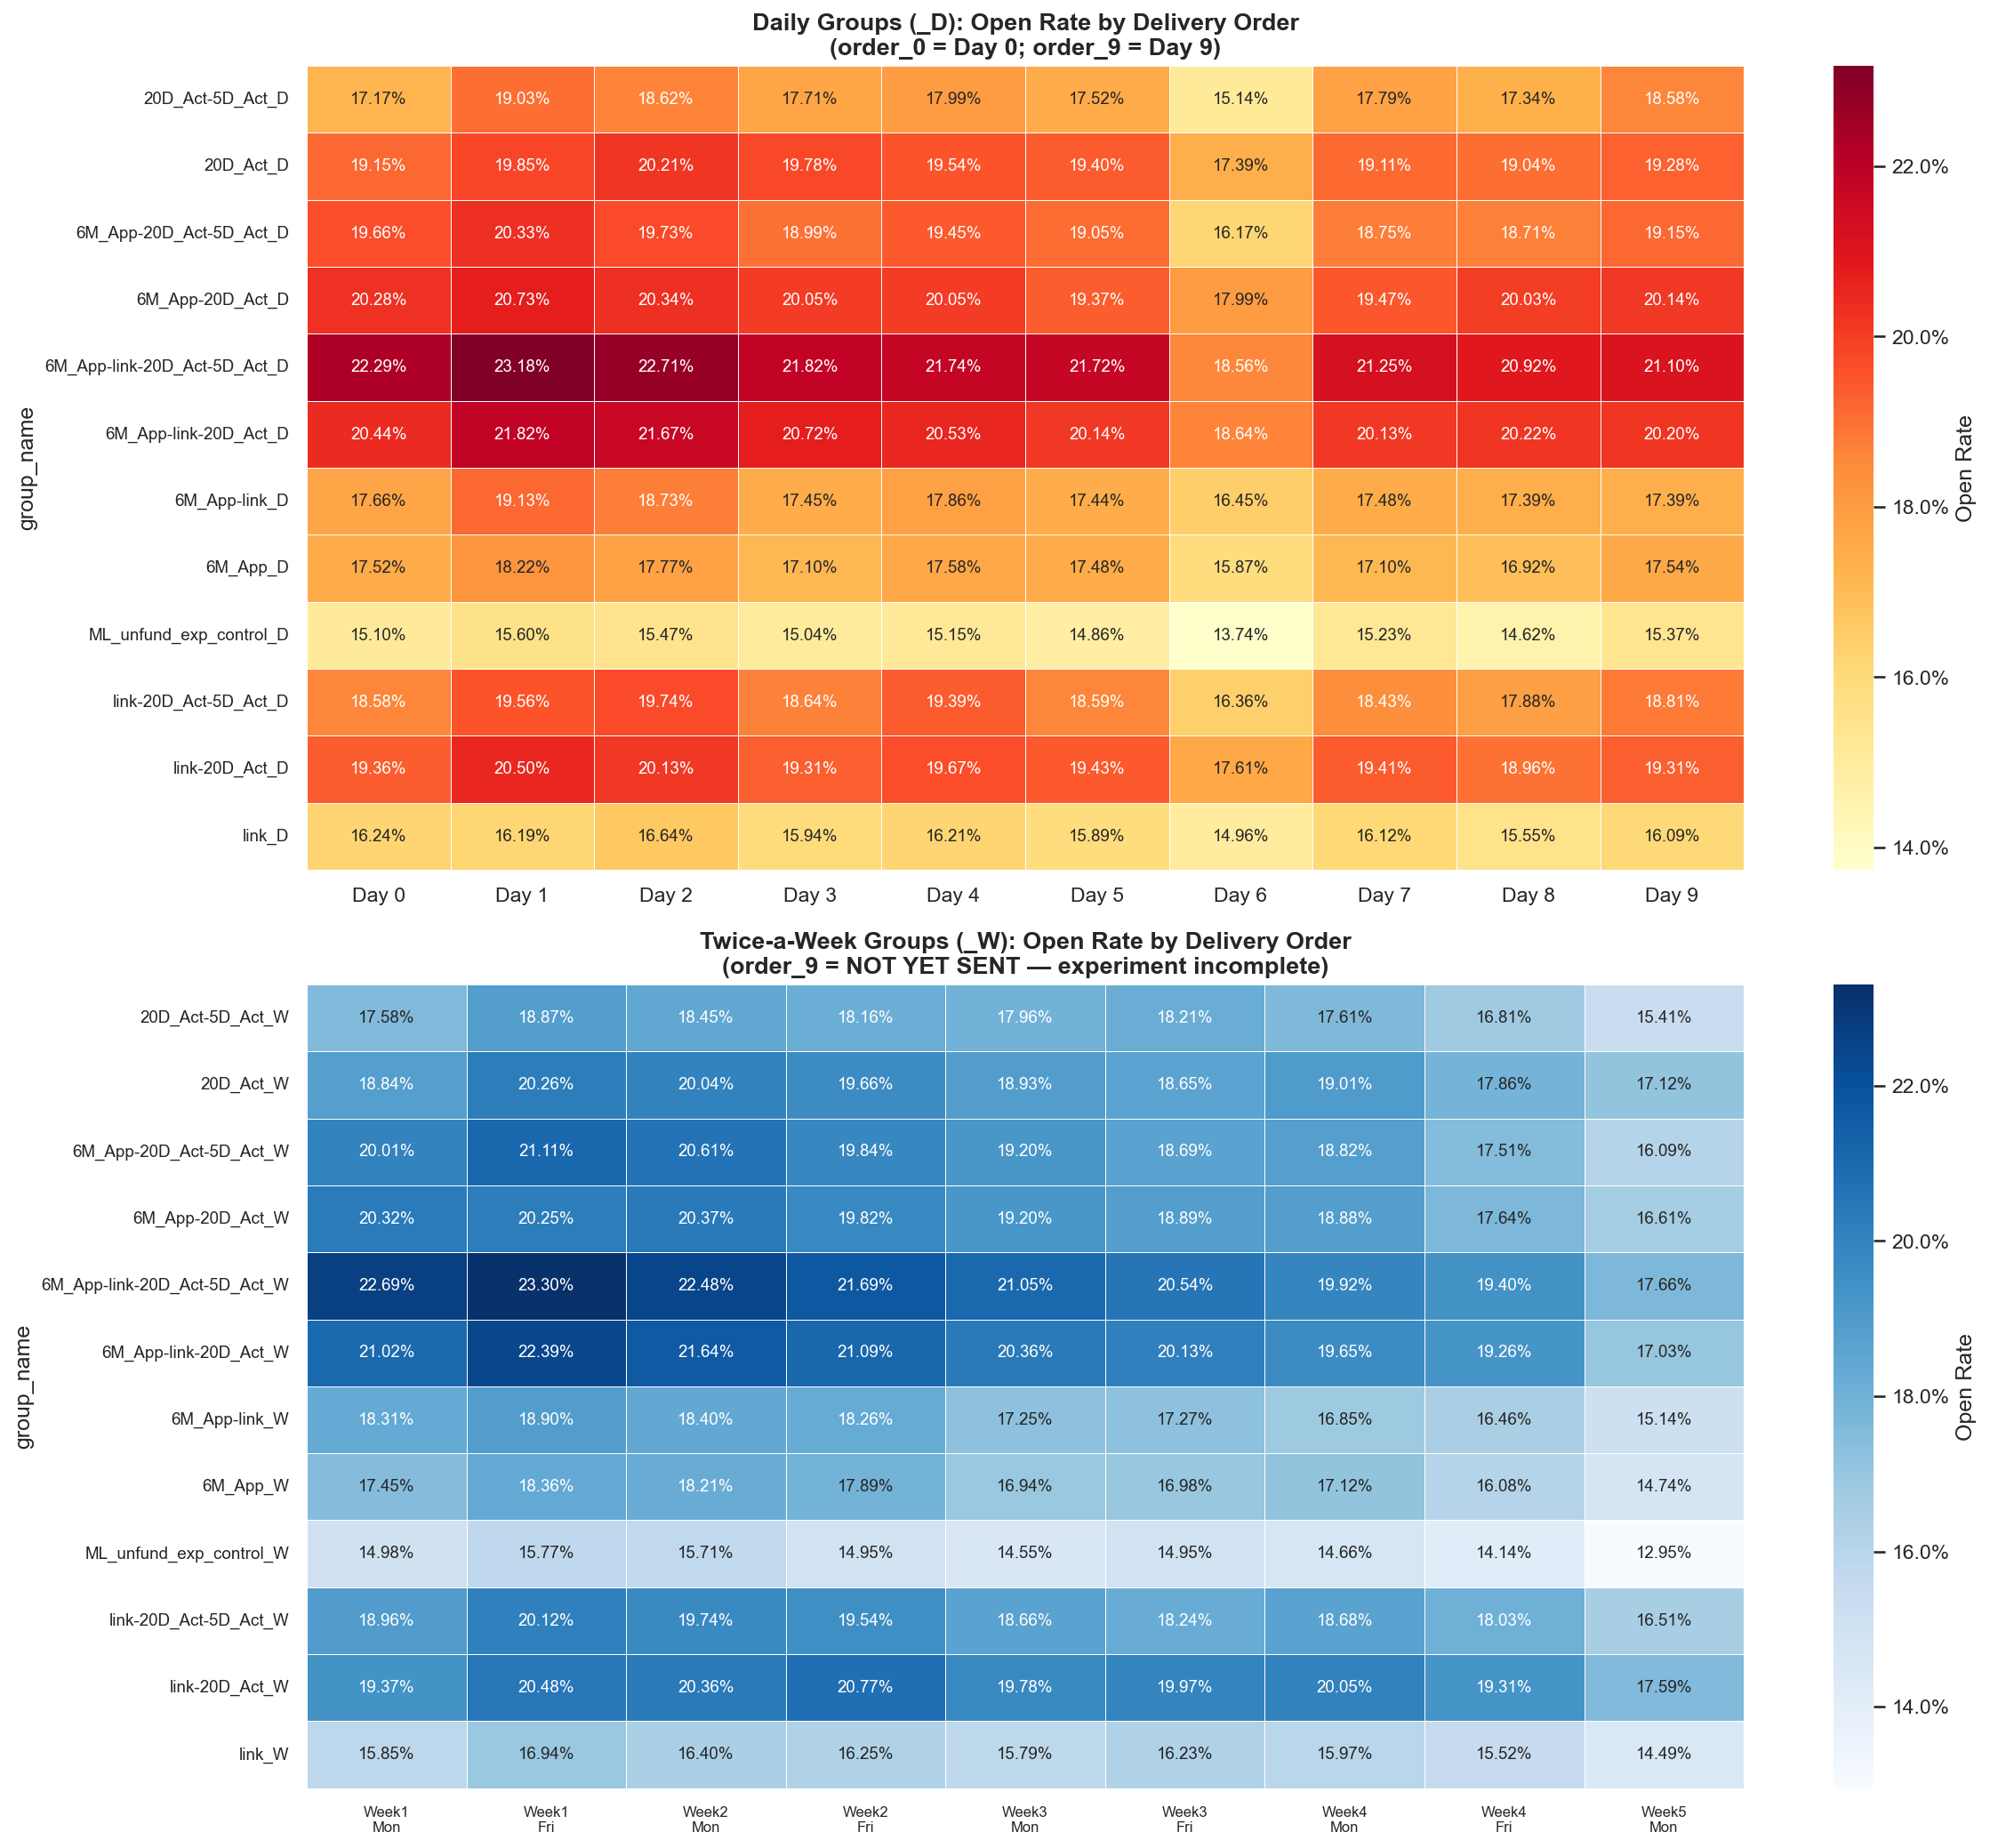
\includegraphics[width=0.82\textwidth]{time_series_open_rate.png}
  \caption{Open rate heatmap by delivery order. Top: Daily groups (experiment complete).
    Bottom: Twice-a-week groups (order\_9 pending — experiment not yet complete).}
  \label{fig:time_series}
\end{figure}

\begin{figure}[H]
  \centering
  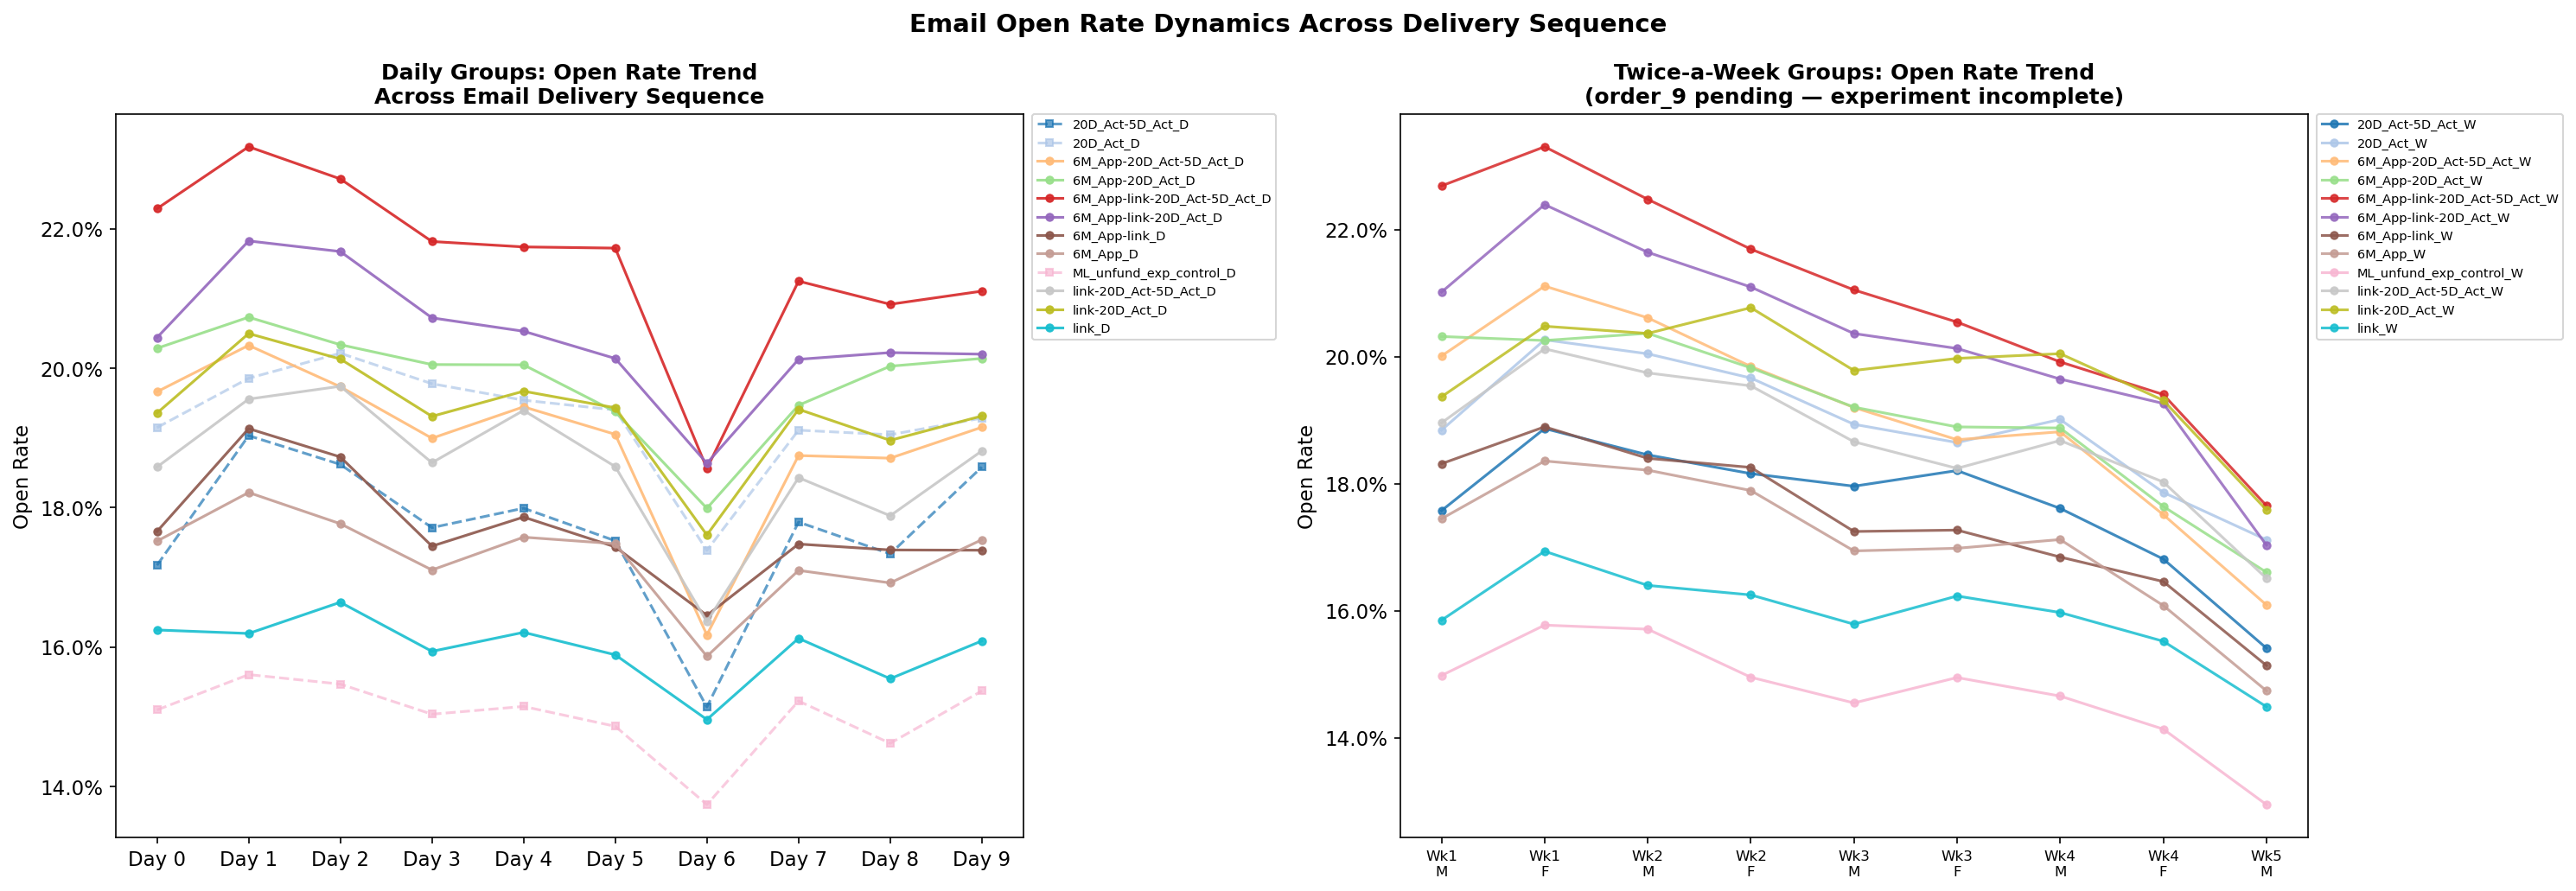
\includegraphics[width=\textwidth]{open_rate_trend.png}
  \caption{Open rate trend curves across the email delivery sequence. The second email
    (order\_1) consistently shows higher engagement than the first (order\_0).}
  \label{fig:open_rate_trend}
\end{figure}

\subsection{Key Findings}

\textbf{Finding 1 — Day 0 does NOT always have the highest open rate.}
Contrary to the novelty hypothesis, \textbf{order\_1 (the second email) consistently
outperforms order\_0 (the first email) across all daily groups}. Average open rates:
order\_0 $\approx$ 18.0\%, order\_1 $\approx$ 19.0\%. This represents a
consistent $\sim$1 percentage point lift.

\textbf{Interpretation — Priming Effect}: The first email ``primes'' the user —
they see the sender, recognize the platform, and consciously or subconsciously
become more receptive to the next communication. This is analogous to the
\textit{mere exposure effect} in psychology: familiarity increases positive response.

\textbf{Finding 2 — Open rates stabilize after the second email, then gradually decline.}
After the order\_1 peak, open rates follow a gentle downward trend through order\_8
and order\_9, suggesting \textbf{email fatigue} accumulates over the 10-email sequence.
However, the decline is moderate (not catastrophic), suggesting the audience remains
engaged throughout.

\textbf{Finding 3 — The experiment is NOT complete for weekly groups.}
The weekly (\texttt{\_W}) groups have zero deliveries recorded for order\_9 (the final
email, scheduled for Day\_32). This is confirmed in the delivery count data:
$\sum_{\text{weekly groups}} N_{\text{order\_9}} \approx 4$ (vs.\ expected $\sim$200,000).

This means \textbf{any analysis of weekly groups at the current snapshot is inherently
incomplete} and final conclusions for weekly delivery arms should be deferred until
the Day\_32 email is sent and a 2-week post-experiment observation window elapses.

\subsection{Strategic Implications for Email Cadence}

Based on these findings, we recommend the following email sequencing strategy for
future campaigns:

\begin{enumerate}[leftmargin=2em]
  \item \textbf{Front-load the sequence}: Send 2--3 emails in the first week to
    capitalize on the priming effect. The jump from order\_0 to order\_1 provides
    the highest engagement gain with the lowest marginal cost.
  \item \textbf{Taper after the third email}: Shift to weekly cadence after the
    initial burst to balance engagement maintenance against fatigue and unsubscribe risk.
  \item \textbf{Template ordering is a lever}: Since order\_1 consistently
    outperforms order\_0, placing the strongest template (FAQ) at position 1 rather
    than position 0 may further amplify the priming effect.
\end{enumerate}

\clearpage
% ─────────────────────────────────────────────────────────────────────────────
\section{Funnel Analysis: Email Open \texorpdfstring{$\to$}{→} Link \texorpdfstring{$\to$}{→} Fund}
% ─────────────────────────────────────────────────────────────────────────────

\subsection{Conversion Funnel Framework}

The conversion funnel maps the sequential steps from initial email contact to
ultimate business outcome:

\begin{equation}
  \underbrace{\text{Email Delivered}}_{\text{100\%}}
  \to
  \underbrace{\text{Email Opened}}_{\sim 18\%}
  \to
  \underbrace{\text{Bank Account Linked}}_{\text{varies by segment}}
  \to
  \underbrace{\text{Account Funded}}_{\sim 3\%}
\end{equation}

\begin{figure}[H]
  \centering
  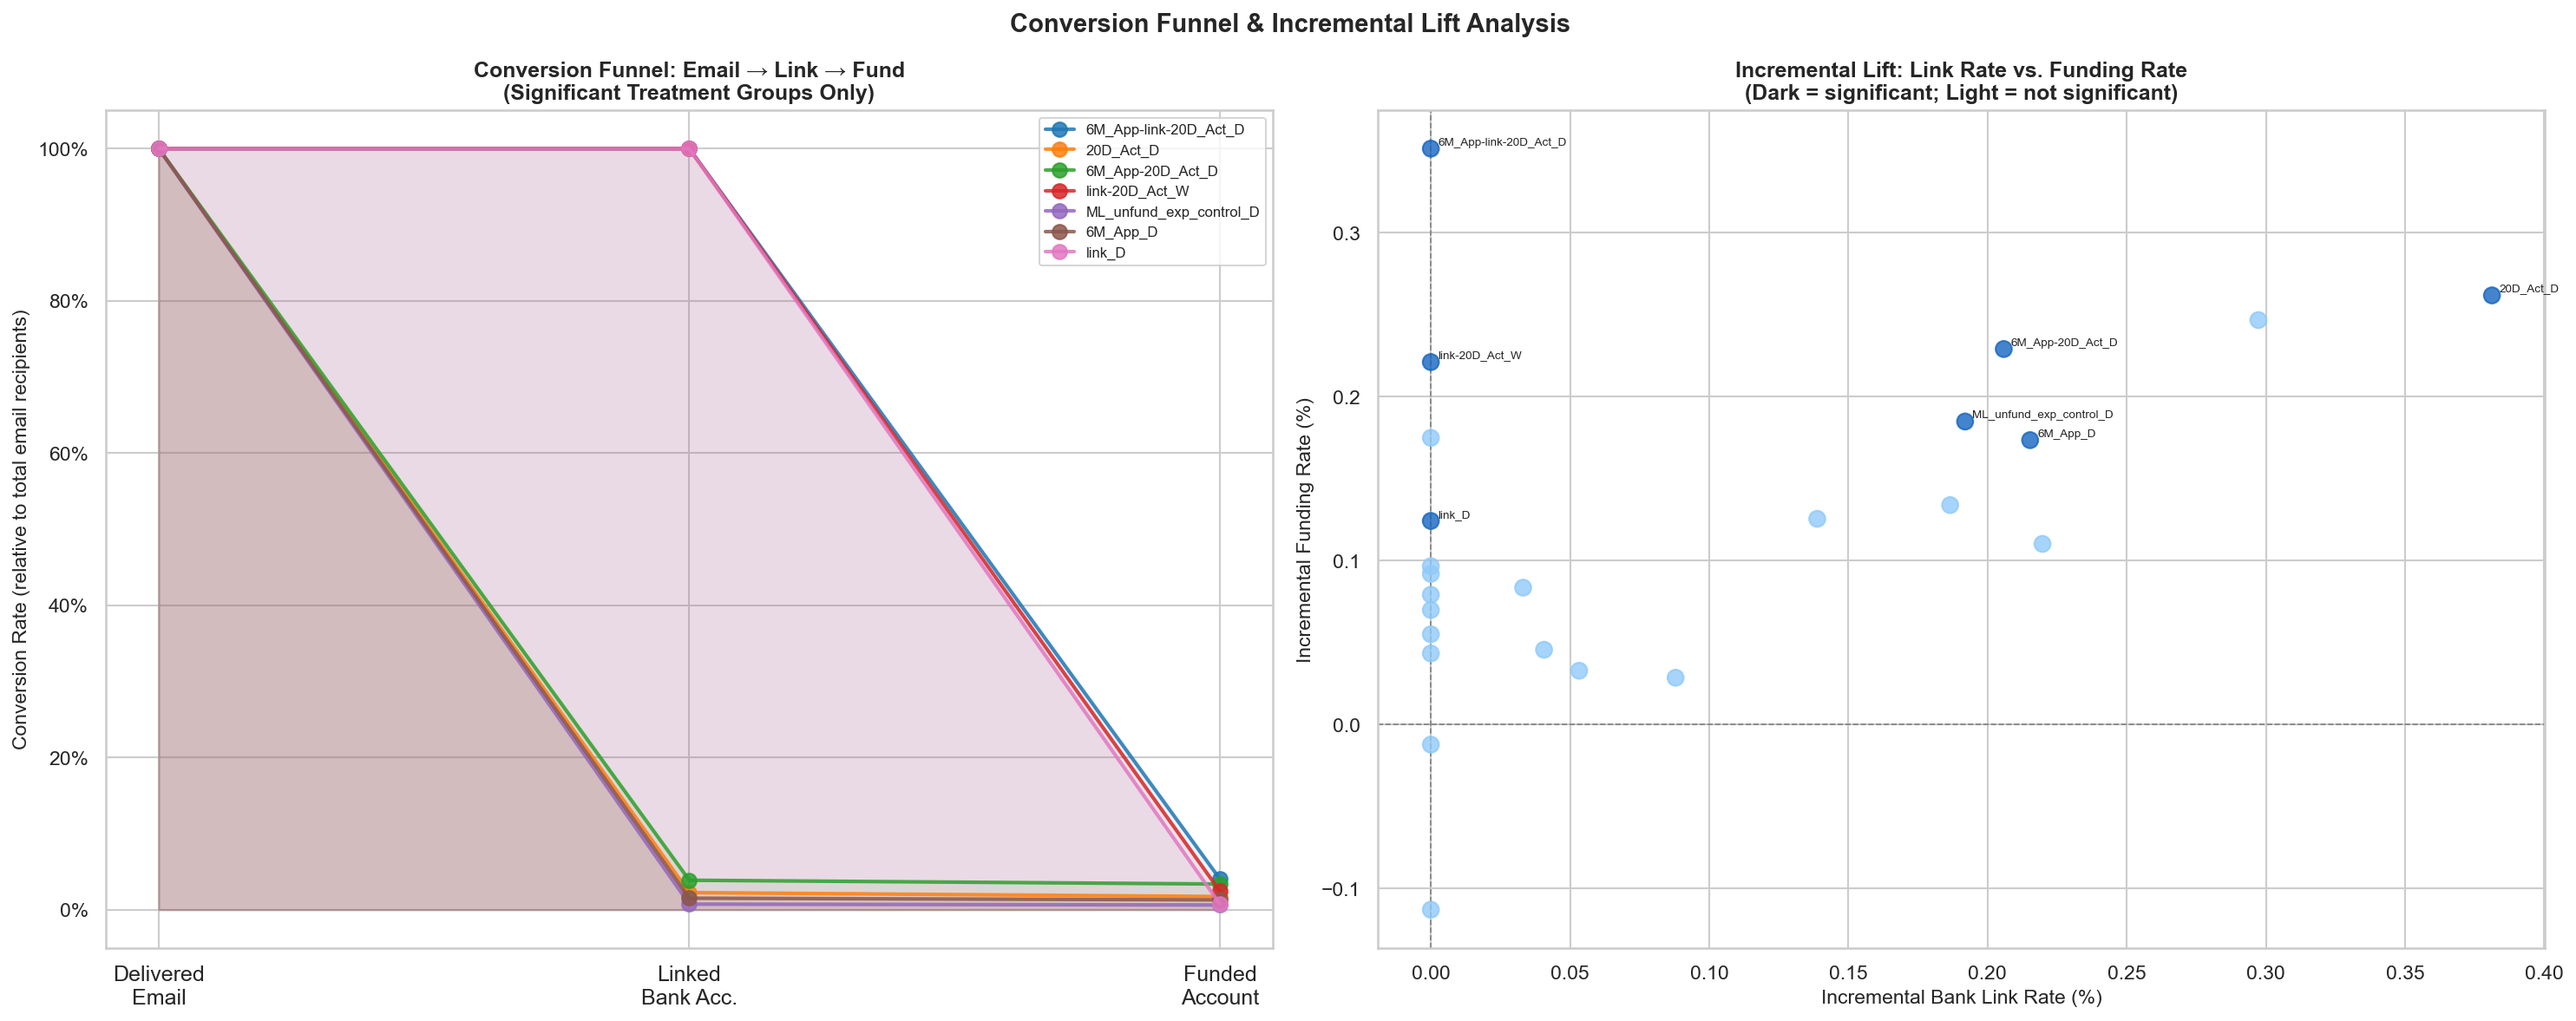
\includegraphics[width=0.88\textwidth]{funnel_analysis.png}
  \caption{Left: Conversion funnel curves for statistically significant treatment groups.
    Right: Incremental lift scatter plot — groups in the upper-right quadrant show the
    highest email-attributable gains in both link and funding rates.}
  \label{fig:funnel}
\end{figure}

\subsection{Funnel Insights}

\textbf{Insight 1 — Bank linkage is a leading indicator for funding.}
Across all groups, users who link their bank account convert to funding at much higher
rates than those who don't. The \texttt{link\_flag} segment, where all users have
already linked accounts, shows a clear advantage — the largest conversion bottleneck
for these users is awareness and motivation, not operational friction.

\textbf{Insight 2 — Email-attributable link uplift correlates with funding uplift.}
The scatter plot (Figure~\ref{fig:funnel}, right) shows a positive relationship
between incremental link rate and incremental funding rate across significant groups.
This validates the causal chain: emails $\to$ higher bank linkage $\to$ higher funding.

\textbf{Insight 3 — Highest-baseline groups are over-represented in non-significant results.}
Groups like \texttt{6M\_App-link-20D\_Act-5D\_Act} have extremely high baseline
funding rates but do not show significant email lift. These users are already
highly motivated — the email provides no meaningful incremental nudge. This argues
for \textbf{segment-specific investment allocation}: email budget should flow toward
medium-intent segments where activation energy is achievable, not high-intent segments
who convert organically.

\clearpage
% ─────────────────────────────────────────────────────────────────────────────
\section{Business Recommendations \& Next Steps}
% ─────────────────────────────────────────────────────────────────────────────

\subsection{Immediate Actions (Post-Experiment)}

\begin{enumerate}[leftmargin=2em, label=\textbf{\arabic*.}]

  \item \textbf{Scale daily delivery to significant treatment groups.}
    The following segments are confirmed to respond positively to daily email campaigns
    and should be included in the next production email run:
    \texttt{20D\_Act\_D}, \texttt{6M\_App\_D}, \texttt{6M\_App-20D\_Act\_D},
    \texttt{6M\_App-link-20D\_Act\_D}, \texttt{ML\_unfund\_exp\_control\_D},
    \texttt{link\_D}.

  \item \textbf{Prioritize \texttt{ml\_funding\_faq} as the anchor template.}
    Given its dominant open rate ($\sim$31.5\%), this template should be placed at
    \textbf{position 1} in the delivery sequence (leveraging the priming effect) and
    potentially personalized further with segment-specific FAQ content.

  \item \textbf{Reduce email exposure for high-baseline, non-significant segments.}
    Segments such as \texttt{6M\_App-link-20D\_Act-5D\_Act} convert organically.
    Email exposure here creates unsubscribe risk without incremental benefit.
    Redirect these users to in-app notifications or push campaigns.

\end{enumerate}

\subsection{Near-Term Optimization (30-60 Days)}

\begin{enumerate}[leftmargin=2em, label=\textbf{\arabic*.}]
  \setcounter{enumi}{3}

  \item \textbf{A/B test subject line variations for \texttt{ml\_funding\_faq}.}
    The template's content clearly resonates, but the open rate may be further
    improved by optimizing the subject line for different segments. Recommended
    subject line hypothesis: segment-specific questions (e.g., ``How do you fund
    your [Segment Name] account? 3 questions answered'').

  \item \textbf{Explore optimal send time.}
    All emails in this experiment were sent between 10:00--10:30 AM. A/B testing
    evening send windows (6:00--8:00 PM) may improve open rates for users who check
    email during commute or evening relaxation time.

  \item \textbf{Implement re-engagement trigger for openers who didn't fund.}
    Users who opened 2+ emails but did not fund within 72 hours represent a
    ``high-intent, unresolved'' cohort. A triggered push notification or in-app
    message at the 72-hour mark may convert this population efficiently.

\end{enumerate}

\subsection{Long-Term Strategic Direction}

\begin{enumerate}[leftmargin=2em, label=\textbf{\arabic*.}]
  \setcounter{enumi}{6}

  \item \textbf{Build a personalized email sequencing model.}
    The current experiment uses randomized email ordering to explore the full
    combinatorial space. The next step is training an ML model (e.g., multi-armed
    bandit or contextual bandits) to dynamically select the next-best email for
    each user based on their engagement history, segment features, and predicted
    conversion probability.

  \item \textbf{Extend to multi-channel orchestration.}
    Email is one channel in a broader engagement stack. Coordinating email
    campaigns with push notifications, in-app banners, and SMS (for high-intent
    moments) can create a multiplicative engagement effect. The segment-level
    insights from this experiment provide a rigorous foundation for cross-channel
    targeting logic.

\end{enumerate}

\clearpage
% ─────────────────────────────────────────────────────────────────────────────
\section{Conclusion}
% ─────────────────────────────────────────────────────────────────────────────

This experiment provides rigorous, statistically-grounded evidence that targeted
email campaigns can causally improve funding rates for approved-but-unfunded fintech
users. Key conclusions:

\begin{itemize}[leftmargin=2em]
  \item \textbf{7 of 24 treatment arms achieve statistical significance} ($p \leq 0.05$),
    generating an estimated $\mathbf{500+}$ email-attributable funded accounts.

  \item \textbf{Daily delivery dominates twice-a-week delivery} for unfunded user
    activation. Frequency is a significant lever independent of content quality.

  \item \textbf{FAQ-style content that directly addresses funding concerns} (the
    \texttt{ml\_funding\_faq} template) outperforms motivational, educational, and
    app-exploration content by a substantial margin, consistent with the hypothesis
    that knowledge barriers are the primary obstacle.

  \item \textbf{The second email in sequence (order\_1) outperforms the first (order\_0)},
    invalidating the novelty hypothesis and suggesting a priming effect. Email
    sequences should be designed to capitalize on this by placing key content at
    position 1 rather than position 0.

  \item \textbf{High-intent segments exhibit diminishing email returns} and should
    be targeted via more frictionless channels (in-app, push) to avoid deliverability
    erosion.

  \item \textbf{The experiment is not yet complete for weekly groups} — final
    conclusions for twice-a-week delivery arms must await the Day\_32 email delivery
    and the post-experiment observation window.

\end{itemize}

The analytical framework established in this project — stratified segmentation,
multi-arm A/B testing with matched controls, causal attribution via proportions
z-tests, and time-series engagement analysis — provides a replicable template for
future growth experiments at scale.

\clearpage
% ─────────────────────────────────────────────────────────────────────────────
\phantomsection
\addcontentsline{toc}{section}{Appendix: Technical Implementation Notes}
\section*{Appendix: Technical Implementation Notes}
% ─────────────────────────────────────────────────────────────────────────────

\subsection*{A. Statistical Test Selection}

We use a \textbf{one-sided proportions Z-test} (rather than a two-sided test) because
our directional hypothesis is specifically that email intervention \textit{increases}
funding rate. Using a one-sided test is appropriate here since:

\begin{enumerate}[leftmargin=2em]
  \item The business question is directional: we seek to confirm positive impact.
  \item A two-sided test would sacrifice statistical power for detecting increases.
  \item The control comparison provides a clean counterfactual (not a pre/post design).
\end{enumerate}

The test is implemented via \texttt{statsmodels.stats.proportion.proportions\_ztest}
with \texttt{alternative='larger'}.

\subsection*{B. Control Group Matching}

Weekly (\texttt{\_W}) treatment groups are matched to the daily (\texttt{\_D}) control
baseline of the same segment. This is because control groups are maintained at the
segment level (not frequency level) — the control users simply do not receive any
emails regardless of what frequency they would have been assigned to.

\subsection*{C. Open Rate Computation Caveat}

Open rate is computed from the \textit{summary status} in \texttt{user\_events.csv},
where each user carries the highest-intent action status for each email. This means
``delivered'' includes all users who received the email but did not open it. The
resulting open rates are user-level open rates (not impression-level), which is the
correct metric for behavioral analysis.

\subsection*{D. Time Series Vectorized Computation}

The time series analysis requires a ``gather'' operation: for each user at
delivery position $d$, look up the email status for whichever template was assigned
at that position. This is implemented via a vectorized mask loop over the
10 email templates to avoid the performance penalty of row-wise \texttt{apply}.

\clearpage
% ─────────────────────────────────────────────────────────────────────────────
% References
% ─────────────────────────────────────────────────────────────────────────────
\begin{thebibliography}{9}

\bibitem{kohavi2009}
  Kohavi, R., Longbotham, R., Sommerfield, D., \& Henne, R. M. (2009).
  Controlled experiments on the web: survey and practical guide.
  \textit{Data Mining and Knowledge Discovery}, 18(1), 140--181.

\bibitem{kohavi2020}
  Kohavi, R., Tang, D., \& Xu, Y. (2020).
  \textit{Trustworthy Online Controlled Experiments: A Practical Guide to A/B Testing}.
  Cambridge University Press.

\bibitem{larsen2023}
  Larsen, N., Stallrich, J., Krishnamurthy, S., Deng, A., Kohavi, R., \& Stevens, N. T. (2023).
  Statistical challenges in online controlled experiments: a review of A/B testing methodology.
  \textit{The American Statistician}, 77(2), 135--149.

\bibitem{email_benchmarks}
  Mailchimp. (2021).
  \textit{Email Marketing Benchmarks and Statistics by Industry}.
  Retrieved from Mailchimp Industry Reports.

\end{thebibliography}

\vspace{2cm}
\hrule
\vspace{0.5cm}
\begin{center}
  \small
  \textit{Data Science Team — Growth \& Engagement} \\
  \textit{Experiment Period: 2020-11-30 through 2021-01-14} \\
  \textit{Report Compiled: February 2021}
\end{center}

\end{document}
